\setchapterpreamble[u]{\margintoc} 
\chapter{Modéliser un SLCI} 
\section{Analyser un asservissement, proposer une structure d'asservissement} 
\section{Modéliser un SLCI en utilisant la transformée de Laplace} 
\graphicspath{{\repStyle/png/}{../SLCI/SLCI-02-FT/51_MCC/images/}} 
\normaltrue \difficilefalse \tdifficilefalse
\correctiontrue

%\UPSTIidClasse{11} % 11 sup, 12 spé
%\newcommand{\UPSTIidClasse}{11}

\exer{Moteur à courant continu$\star$ \label{B2:04:51}}
\setcounter{question}{0}\UPSTIcompetence[2]{B2-04}
\index{Compétence B2-04}
\index{Fonctions de transfert}
\index{Moteur à courant continu}
\index{MCC}
\ifcorrection
\else
\marginnote{\textbf{Pas de corrigé pour cet exercice.}}
\fi


\ifprof 
\else
On donne les équations du moteur à courant continu :
\begin{itemize}
\item $u(t) = e(t)+ Ri(t) +L \dfrac{\text{d}i(t)}{\text{d} t}$;
\item $e(t)=K\omega(t)$;
\item $c(t)=Ki(t)$;
\item $c(t)- f\omega(t)=J\dfrac{\text{d}\omega(t)}{\text{d} t}$.
\end{itemize}
\fi

\question{Exprimer la fonction de transfert $H(p)=\dfrac{\Omega(p)}{U(p)}$.}
\ifprof
En passant les équations dans le domaine de Laplace, on a : 
\begin{itemize}
\item $U(p) = E(p)+ RI(p) +LpI(p)$;
\item $E(p)=K_m\Omega(p)$;
\item $C(p)=K_mI(p)$;
\item $C(p)- f\Omega(p)=Jp\Omega(p)$ $\Leftrightarrow C(p)=\Omega(p)\left( Jp +f \right)$.
\end{itemize}

\textbf{Vous devez savoir qu'un moteur à courant continu est piloté en tension ($U(p)$) et qu'en sortie on observe le taux de rotation ($\Omega(p)$). }

En ne conservant que $U(p)$ et $\Omega(p)$, on a donc
$U(p) = E(p)+ RI(p) +LpI(p)$
$ \Leftrightarrow U(p) = K_m\Omega(p)+ \left(R +Lp\right)\dfrac{C(p)}{K_m}$
$ \Leftrightarrow U(p) = K_m\Omega(p)+ \left(R +Lp\right)\dfrac{\Omega(p)\left( Jp +f \right)}{K_m}$
$ \Leftrightarrow U(p) = \left(K_m+ \left(R +Lp\right)\dfrac{\left( Jp +f \right)}{K_m}\right)\Omega(p)$
$ \Leftrightarrow U(p) =  \dfrac{K_m^2 + \left(R +Lp\right)\left( Jp +f \right)}{K_m}\Omega(p)$.

On a donc $H(p)=\dfrac{\Omega(p)}{U(p)}$ $=\dfrac{K}{K^2 +\left(R +Lp\right) \left( Jp +f \right)} $.

%\begin{figure}[H]
%\centering
%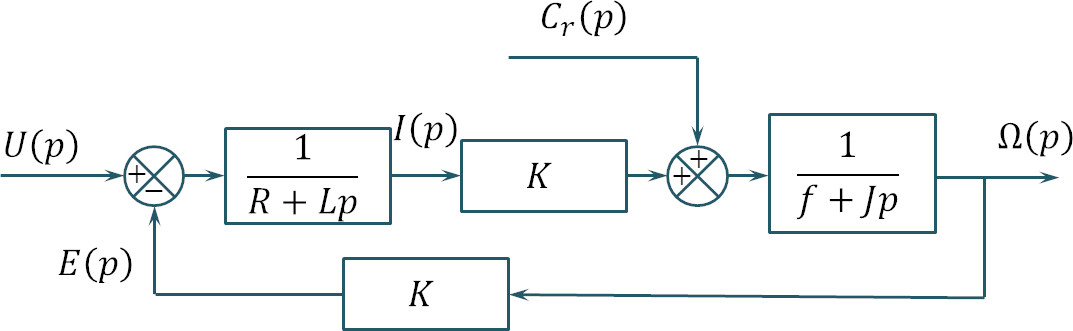
\includegraphics[width=\linewidth]{51_01_c}
%\caption{Évolution du couple utile en fonction de la vitesse de rotation pour des
%fréquences de commande de \SI{90}{Hz} à \SI{110}{Hz}. \label{fig_50_04}}
%\end{figure}
\else
\fi

\question{Préciser l'ordre et la classe de $H$.}
\ifprof
$H$ est d'ordre 2 et de classe 0 car on ne peut pas mettre de $p$ en facteur. Le terme de plus haut degré du dénominateur est de degré 2. 
\else
\fi

\question{Mettre $H(p)$ sous forme canonique.}
\ifprof
$H(p)=\dfrac{K_m}{K_m^2+ Rf +\left(RJ  + Lf\right) p + LJp^2 } $
$\Leftrightarrow H(p)=\dfrac{\dfrac{K_m}{K_m^2+ Rf}}{1 +\dfrac{\left(RJ  + Lf\right)}{K_m^2+ Rf} p + \dfrac{LJ}{K_m^2+ Rf}p^2 } $. 

\else
\fi




\question{Donner les caractéristiques de la fonction de transfert.}
\ifprof
En identifiant avec la forme canonique standard, $H(p)=\ordredeux$ soit
$K = \dfrac{K_m}{K_m^2+ Rf}$, $\dfrac{2\xi}{\omega_0} = \dfrac{\left(RJ  + Lf\right)}{K_m^2+ Rf}$ et $\dfrac{1}{\omega_0^2}=\dfrac{LJ}{K_m^2+ Rf}$.


Au final,
$K = \dfrac{K_m}{K_m^2+ Rf}$,
$\omega_0=\sqrt{\dfrac{K_m^2+ Rf}{LJ}}$,
$\xi = \dfrac{RJ  + Lf}{2\sqrt{{LJ\left(K_m^2+ Rf\right)}}}$.
\else
\fi

\question{Vérifier l'homgénéité des différentes constantes.}
\ifprof

Le gain doit être en $\si{rad.s^{-1}V^{-1}}$.

D'une part, $[K_m]=\si{N.m.A^{-1}}$. D'autre part, $[K_m]=\si{V.rad^{-1}.s}$. On a donc $\si{V.rad^{-1}.s}=\si{N.m.A^{-1}}$. (On pourrait aussi le montrer par une analyse dimensionnelle...)

De plus $[R]=\Omega = \dfrac{\si{V}}{\si{A}}$ et $[f]=\si{N.m.rad^{-1}.s}$.

On a donc 
$[K]=\dfrac{\si{N.m.A^{-1}}}
{(\si{N.m.A^{-1}})^2+\si{N.m.rad^{-1}.s}\times\si{VA^{-1}} }$
$=\dfrac{1}
{\si{N.m.A^{-1}}+\si{rad^{-1}.s.V} }$
$=\dfrac{1} {\si{rad^{-1}.s.V} }$
$= {\si{rad.s^{-1}.V^{-1}} }$. 

\vspace{.5cm}

La pulsation propre doit être en $\si{s^{-1}}$ ou $\si{rad.s^{-1}}$.

On a vu que $[K_m^2] = [Rf]$. De plus $[L] = H =  \si{V.s.A^{-1}}$ et 
$[J]=\si{Nm.rad^{-1}s^2}$ (PFD).

$[\omega_0]=\sqrt{
\dfrac{\si{N^2.m^2.A^{-2}}}
{\si{V.s.A^{-1}} \times \si{Nm.rad^{-1}s^2}}
}$
$=\sqrt{
\dfrac{\si{N.m.rad}}{\si{V.s.A.s^2}}
}$. 
Or, $\si{W}=\si{N.m.rad.s^{-1}}=\si{VA}$.

On a alors 
$[\omega_0]=\sqrt{
\dfrac{\si{N.m.rad.s^{-1}}}{\si{V.s^2.A}}
}$
$=\sqrt{
\dfrac{1}{\si{s^2}}
}=\si{s^{-1}}$.


Enfin, $\xi$ est sans unité... à vérifier :)
%
%
%
%$[\xi]=  \dfrac{\si{N.m.rad^{-1}.s}\si{Nm.rad^{-1}s^2}  + \si{V.s.A^{-1}}\si{N.m.rad^{-1}.s}}{\sqrt{{\si{V.s.A^{-1}}\si{Nm.rad^{-1}s^2} \si{N.m.rad^{-1}.s}\si{N.m.rad^{-1}.s}}}}$
%$=  \dfrac{\si{N.m.rad^{-1}.s}\si{Nm.rad^{-1}s^2}  + \si{V.s.A^{-1}}\si{N.m.rad^{-1}.s}}{\si{N.m.rad^{-1}.s}\sqrt{{\si{V.s.A^{-1}}\si{Nm.rad^{-1}s^2} }}}$
%$=  \dfrac{\si{Nm.rad^{-1}s^2}  + \si{V.s.A^{-1}}}
%{\sqrt{{\si{V.s.A^{-1}}\si{Nm.rad^{-1}s^2} }}}$.
%
%Or, $\si{W}=\si{N.m.rad.s^{-1}}=\si{VA}$; donc $\si{N.m}=\si{VA.rad^{-1}.s}$; donc 
%
%
%$[\xi]=  \dfrac{\si{VA.rad^{-1}.s.rad^{-1}s^2}  + \si{V.s.A^{-1}}}
%{\sqrt{{\si{V.s.A^{-1}}\si{VA.rad^{-1}.s.rad^{-1}s^2} }}}$
%$=  \dfrac{\si{VA.rad^{-2}s^3}  + \si{V.s.A^{-1}}}
%{\sqrt{{\si{V^2.rad^{-2}s^4} }}}$
%$=  \dfrac{\si{VA.rad^{-2}s^3}  + \si{V.s.A^{-1}}}
%{\si{V.rad^{-1}s^2} }$
%$=  \dfrac{\si{A.rad^{-2}s^2}  + \si{V.A^{-1}}}
%{\si{rad^{-1}s} }$
%$=  \dfrac{\si{A^2.rad^{-2}s^2}  + \si{V}}
%{\si{A.rad^{-1}s} }$

\else
\fi




\ifprof
\else

\ifcolle
\else
\noindent\footnotesize
\fbox{\parbox{.9\linewidth}{
Éléments de corrigé : 
\begin{enumerate}
    \item $H(p)=\dfrac{K_m}{K_m^2 +\left(R +Lp\right) \left( Jp +f \right)} $.
    \item Ordre 2, classe 0.
    \item $H(p)=\dfrac{\dfrac{K_m}{K_m^2+ Rf}}{1 +\dfrac{\left(RJ  + Lf\right)}{K_m^2+ Rf} p + \dfrac{LJ}{K_m^2+ Rf}p^2 } $.
    \item $K = \dfrac{K_m}{K_m^2+ Rf}$,
$\omega_0=\sqrt{\dfrac{K_m^2+ Rf}{LJ}}$,
$\xi = \dfrac{RJ  + Lf}{2\sqrt{{LJ\left(K_m^2+ Rf\right)}}}$.
\end{enumerate}}}
\normalsize
\fi

\begin{flushright}
\footnotesize{Corrigé  voir \ref{B2:04:51}.}
\end{flushright}%
\fi 
 
\section{Modéliser un SLCI en utilisant un schéma-bloc} 
\graphicspath{{\repStyle/png/}{../SLCI/SLCI-03-SchemaBlocs/39_SeineMusicale/images/}} 
\normaltrue \difficilefalse \tdifficilefalse
\correctiontrue

%\UPSTIidClasse{11} % 11 sup, 12 spé
%\newcommand{\UPSTIidClasse}{11}

\exer{La Seine Musicale$\star$ \label{B2:07:39}}
\setcounter{question}{0}\UPSTIcompetence[2]{B2-07}
\index{Compétence B2-07}
\index{La Seine Musicale}
\ifcorrection
\else
\marginnote{\textbf{Pas de corrigé pour cet exercice.}}
\fi

\ifprof
\else
Soit le schéma-blocs suivant. 
\begin{figure}[H]
\centering
\rotatebox{90}{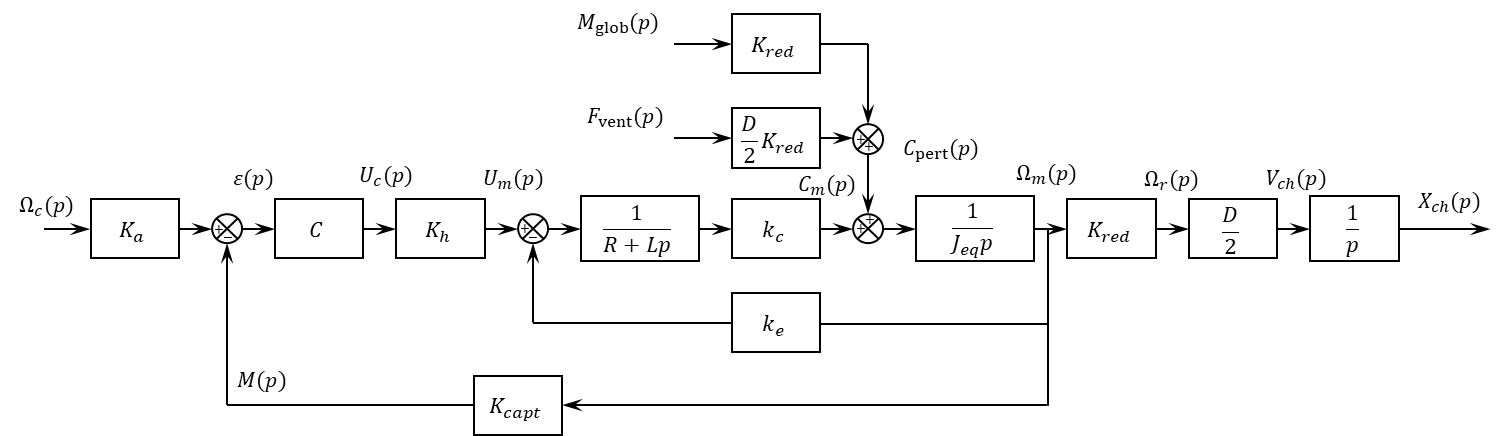
\includegraphics[width=.7\textheight]{39_01}}
%\caption{ \label{fig_39_01}}
\end{figure}
\fi

\question{En considérant que la perturbation $C_{\text{pert}}(p)$ est nulle, déterminer $H_f(p)=\dfrac{\Omega_m(p)}{\Omega_c(p)}$ sous forme canonique.}
\ifprof
Réduction de la boucle du moteur à courant continu : 
$\dfrac{\Omega_m(p)}{U_m(p)}=\dfrac{\dfrac{k_c}{R+Lp}\dfrac{1}{J_{eq}p}}{1+\dfrac{k_c}{R+Lp}\dfrac{k_e}{J_{eq}p}}$
$=\dfrac{k_c}{\left(R+Lp\right)J_{eq}p+k_ek_c}$.

On a alors, 

$
\dfrac{X_{ch}(p)}{\Omega_c(p)} =
K_a  \dfrac{CK_h \dfrac{k_c}{\left(R+Lp\right)J_{eq}p+k_ek_c}}{1+CK_hK_{\text{capt}} \dfrac{k_c}{\left(R+Lp\right)J_{eq}p+k_ek_c}}
$ 

$
=
K_a \dfrac{CK_h k_c}{\left(R+Lp\right)J_{eq}p+k_ek_c+CK_hK_{\text{capt}} k_c}
$

$
=
\dfrac{K_a }{\left( k_ek_c+CK_hK_{\text{capt}} k_c\right)} \dfrac{CK_h k_c}{\dfrac{J_{eq}\left(R+Lp\right)}{k_ek_c+CK_hK_{\text{capt}} k_c}p+1}
$.

\else
\fi

\question{En prenant $\Omega_c(p)=0$, exprimer la fonction de transfert $H_r(p)=\dfrac{\Omega_m(p)}{C_{\text{pert}}(p)}$ en la mettant sous la forme : $H_r(p)=-\dfrac{\alpha \left(1+\tau p\right)}{1+\gamma p+\delta p^2}$. Exprimer $\alpha$, $\tau$, $\gamma$ et $\delta$ en fonction des différents paramètres de l’étude.}
\ifprof ~\\
Par lecture directe du schéma-blocs, on a 
$\Omega_m(p) = \dfrac{1}{J_{eq}p}\left(C_{\text{pert}}(p) + C_m(p)\right)$.

De plus, 
$C_m(p) = \left(U_m(p)-k_e\Omega_m(p)\right) \dfrac{k_c}{R+Lp}$
 et $U_m(p)=\varepsilon(p) C K_h = -\Omega_m(p) C K_h K_{\text{capt}}$.
 
 On a donc, 
 
 $\Omega_m(p) = \dfrac{1}{J_{eq}p} C_{\text{pert}}(p) 
 + \dfrac{1}{J_{eq}p} \left(-\Omega_m(p) C K_h K_{\text{capt}}-k_e\Omega_m(p)\right) \dfrac{k_c}{R+Lp}$.

$\Leftrightarrow 
\Omega_m(p) = \dfrac{1}{J_{eq}p} C_{\text{pert}}(p) 
 + \dfrac{1}{J_{eq}p} \Omega_m(p) \left(- C K_h K_{\text{capt}}-k_e\right) \dfrac{k_c}{R+Lp}$
 
 $\Leftrightarrow 
\Omega_m(p)\left(1+\dfrac{1}{J_{eq}p} \left( C K_h K_{\text{capt}}+k_e\right) \dfrac{k_c}{R+Lp}\right)= \dfrac{1}{J_{eq}p} C_{\text{pert}}(p) 
 $

$\Leftrightarrow 
\dfrac{\Omega_m(p)}{C_{\text{pert}}(p)}
 = \dfrac{\dfrac{1}{J_{eq}p}}{\left(1+\dfrac{1}{J_{eq}p} \left( C K_h K_{\text{capt}}+k_e\right) \dfrac{k_c}{R+Lp}\right)}
 $


$\Leftrightarrow 
\dfrac{\Omega_m(p)}{C_{\text{pert}}(p)}
 = \dfrac{R+Lp}{J_{eq}p\left(R+Lp\right)+ \left( C K_h K_{\text{capt}}+k_e\right) k_c}
 $

$\Leftrightarrow 
\dfrac{\Omega_m(p)}{C_{\text{pert}}(p)}
 = \dfrac{R}{\left( C K_h K_{\text{capt}}+k_e\right) k_c} \dfrac{1+\dfrac{L}{R}p}{\dfrac{J_{eq}}{\left( C K_h K_{\text{capt}}+k_e\right) k_c}p\left(R+Lp\right)+ 1}
 $.
 
 Par identification, on a alors : 
 $\alpha = - \dfrac{R}{\left( C K_h K_{\text{capt}}+k_e\right) k_c}$, 

 $\tau = \dfrac{L}{R}$

$\gamma = \dfrac{R J_{eq}}{\left( C K_h K_{\text{capt}}+k_e\right) k_c} $

$\delta = \dfrac{LJ_{eq}}{\left( C K_h K_{\text{capt}}+k_e\right) k_c}$.

\else
\fi

\question{Exprimer $X_{\text{ch}}(p)$ en fonction de $\Omega_m(p)$ et $C_{\text{pert}}(p)$.}
\ifprof ~\\
D'une part, $\Omega_m(p) = H_f(p) \Omega_c(p)$ quand il n'y a pas de perturbation.
D'autre part, $\Omega_m(p) = H_r(p) C_{\text{pert}}(p)$ quand il n'y a pas de perturbation.

Par superposition, on a donc $\Omega_m(p) = H_f(p) \Omega_c(p) + H_r(p) C_{\text{pert}}(p)$.

Par suite, $X_{ch}(p)=\left(H_f(p) \Omega_c(p) + H_r(p) C_{\text{pert}}(p)\right) \dfrac{DK_{\text{red}}}{2p}$.
\else
\fi



\ifprof
\else
\footnotesize
\noindent \begin{tabular}{|p{.9\linewidth}|}
\hline
Indications : 
\begin{enumerate}
\item $ H_f(p)=
\dfrac{K_a }{\left( k_ek_c+CK_hK_{\text{capt}} k_c\right)} \dfrac{CK_h k_c}{\dfrac{J_{eq}\left(R+Lp\right)}{k_ek_c+CK_hK_{\text{capt}} k_c}p+1} $.
\item  $\alpha = - \dfrac{R}{\left( C K_h K_{\text{capt}}+k_e\right) k_c}$,  $\tau = \dfrac{L}{R}$, 
$\gamma = \dfrac{R J_{eq}}{\left( C K_h K_{\text{capt}}+k_e\right) k_c} $, 
$\delta = \dfrac{LJ_{eq}}{\left( C K_h K_{\text{capt}}+k_e\right) k_c}$.
\item $X_{ch}(p)=\left(H_f(p) \Omega_c(p) + H_r(p) C_{\text{pert}}(p)\right) \dfrac{DK_{\text{red}}}{2p}$.
\end{enumerate}
\\ \hline
\end{tabular}
\normalsize

\begin{flushright}
\footnotesize{Corrigé  voir \ref{B2:07:39}.}
\end{flushright}%
\fi 
 
\graphicspath{{\repStyle/png/}{../SLCI/SLCI-03-SchemaBlocs/47_SysReeduc/images/}} 
\normaltrue \difficilefalse \tdifficilefalse
\correctiontrue
%\UPSTIidClasse{11} % 11 sup, 12 spé
%\newcommand{\UPSTIidClasse}{11}

\exer{Machine de rééducation SysReeduc $\star$ \label{B2:07:47}}
\setcounter{question}{0}\marginnote{\xpComp{SLCI}{03}}%\UPSTIcompetence{B2-07}
\index{Compétence B2-07}\index{Compétence SLCI-03}
\index{Machine de rééducation SysReeduc}
\index{Schéma-blocs}
\ifcorrection
\else
\marginnote{\textbf{Pas de corrigé pour cet exercice.}}
\fi



\ifprof
\else
On propose une modélisation par schéma-blocs dans la figure suivante. 
\begin{figure}[!h]
\centering
{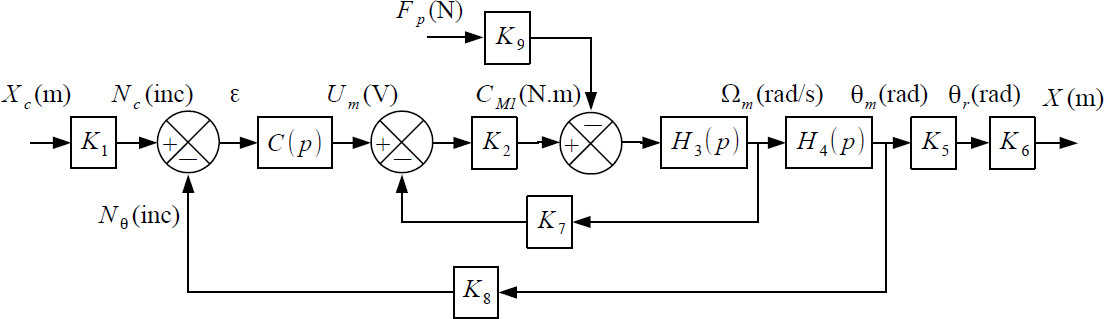
\includegraphics[width=\linewidth]{47_01}}
%\caption{ \label{fig_47_01}}
\end{figure}




Le moteur à courant continu est régi par les équations suivantes :
$ u_m(t)=e(t)+Ri(t)$, $e(t)=k_e\omega_m(t)$ et $C_{M1}(t)=k_t i(t)$. 

Une étude dynamique a mené à l'équation suivante : 
$$\left(M+m\right)r\rho_1 \dot{\omega}_m(t)=\dfrac{C_{M1}(t)}{\rho_1 r}-F_p(t)$$ avec : $M$ la masse du chariot et $m$ la masse du support de pied, $\rho_1=\dfrac{1}{10}$ le rapport de réduction du réducteur, $r=\SI{46,1}{mm}$ le rayon de la poulie du transmetteur poulie--courroie, $C_{M1}(t)$ le couple délivré par le moteur et $F_p(t)$ l'effort délivré par le patient sur le support 3. 

Le codeur incrémental possède 500 fentes équiréparties. Deux émetteurs-récepteurs positionnés en quadrature permettent de mesurer l'information. 
\fi

\question{À partir des équations proposées, déterminer les fonctions de transfert $K_1$, $K_2$, $H_3(p)$, $H_4(p)$,  $K_5$, $K_6$, $K_7$, $K_8$ et $K_9$.}
\ifprof
%\begin{corrige}
~\\
On a :
\begin{itemize}
\item $ u_m(t)=e(t)+Ri(t) \Rightarrow  U_m(p)=E(p)+RI(p) $ et $C_{M1}(p)=k_t I(p)$ donc $K_2 = \dfrac{k_t}{R}$;
\item $E(p)=k_e\Omega_m(p)$ et donc $K_7 = k_e$;
\item $\left(M+m\right)r\rho_1 p\Omega_m(p)=\dfrac{C_{M1}(p)}{\rho_1 r}-F_p(p) \Leftrightarrow\left(M+m\right)r^2\rho_1^2 p\Omega_m(p)=C_{M1}(p)-\rho_1 rF_p(p) $ et donc $K_9 = \rho_1 r$ et $H_3(p)=\dfrac{1}{\left(M+m\right)r^2\rho_1^2 p}$;
\item  $H_4(p)$ permet d'obtenir une position à partir d'une vitesse. Il s'agit donc d'un intégrateur et $H_4(p)=\dfrac{1}{p}$; 
\item un codeur incrémental avec 1 émetteur-récepteur permet de détecter les fentes et les << non fentes >> donc ici 1000 informations par tour. Avec un second émetteur, on double la résolution soit 2000 informations pour un tour soit $K_8  = \dfrac{2000}{2\pi}$;
\item en utilisant le réducteur et le poulie courroie, on a directement $K_5=\rho_1$ et $K_6=r$ (à convertir en mètres);
\item enfin, $K_1$ convertit des mètres en incréments. $X_c$ est la consigne que doit respectée $X$. Pour avoir un asservissement précis, il faut donc $\varepsilon = 0$ et $X=X_c$ soit $\varepsilon = 0 = K_1 X_C - K_8 \theta_m = K_1 X_C - K_8 \dfrac{X}{K_5 K_6}$. Au final, $K_1 =\dfrac{K_8}{K_5 K_6}$.
\end{itemize}
%\end{corrige}
\else
\fi


\question{Montrer que le schéma-blocs peut être mis sous la forme suivante. On exprimera $A$, $B$ et $D$ en fonction des paramètres du système $r$, $\rho_1$, $k_t$, $k_e$, $R$, $M$, $m$ et $K_8$. }
\ifprof
%\begin{corrige}~\\
D'une part,

$X(p)=\left(\left(X_C(p)-X(p)\right)C(p)-F_P(p) D \right)\dfrac{A}{p\left(Bp+1\right)}$

$X(p)=\dfrac{A\left(X_C(p)-X(p)\right)C(p)}{p\left(Bp+1\right)}- \dfrac{AF_P(p) D}{p\left(Bp+1\right)}$

$\Leftrightarrow X(p)+\dfrac{AX(p)C(p)}{p\left(Bp+1\right)}=\dfrac{AX_C(p)C(p)}{p\left(Bp+1\right)}- \dfrac{AF_P(p) D}{p\left(Bp+1\right)}$.
$\Leftrightarrow X(p)\left(\dfrac{p\left(Bp+1\right)+AC(p)}{p\left(Bp+1\right)}\right)=\dfrac{AX_C(p)C(p)}{p\left(Bp+1\right)}+ \dfrac{AF_P(p) D}{p\left(Bp+1\right)}$

\fbox{$\Leftrightarrow X(p)=\dfrac{AX_C(p)C(p)}{p\left(Bp+1\right)+AC(p)}- \dfrac{AF_P(p) D}{p\left(Bp+1\right)+AC(p)}$.}


D'autre part, 
$X(p)=\Omega_m(p)H_4(p)K_5K_6$, $U_m(p)=\left(X_c(p)K_1 - \theta_m(p)K_8\right)C(p)$, $\theta_m(p)=\Omega_m(p)H_4(p)$. 

$\Omega_m(p) = \left(\left(U_m(p)-\Omega_m(p) K_7\right)K_2- F_P(p)K_9\right)H_3(p)$

$\Leftrightarrow \Omega_m(p) \left(1+K_7K_2H_3(p)\right)= U_m(p)H_3(p)K_2- F_P(p)H_3(p)K_9$


$X(p)=\left( U_m(p)H_3(p)K_2- F_P(p)H_3(p)K_9 \right)\dfrac{H_4(p)K_5K_6}{1+K_7K_2H_3(p)}$

$\Leftrightarrow X(p)=\left( \left(X_c(p)K_1 - \theta_m(p)K_8\right)C(p)H_3(p)K_2- F_P(p)H_3(p)K_9 \right)\dfrac{H_4(p)K_5K_6}{1+K_7K_2H_3(p)}$

$\Leftrightarrow X(p)=\left( \left(X_c(p)K_1 - X(p)\dfrac{K_8}{K_5K_6}\right)C(p)H_3(p)K_2- F_P(p)H_3(p)K_9 \right)\dfrac{H_4(p)K_5K_6}{1+K_7K_2H_3(p)}$

$\Leftrightarrow X(p)=\left(\left(X_c(p) - X(p)\right)C(p)H_3(p)  K_1K_2- F_P(p)H_3(p)K_9 \right)\dfrac{H_4(p)K_5K_6}{1+K_7K_2H_3(p)}$

$\Leftrightarrow X(p)\left( 1+ C(p)H_3(p)  K_1K_2 \dfrac{H_4(p)K_5K_6}{1+K_7K_2H_3(p)}\right)=\left(X_c(p) C(p)H_3(p)  K_1K_2- F_P(p)H_3(p)K_9 \right)\dfrac{H_4(p)K_5K_6}{1+K_7K_2H_3(p)}$


\fbox{$\Leftrightarrow X(p)\left( 1+K_7K_2H_3(p)+ C(p)H_3(p)  K_1K_2 H_4(p)K_5K_6\right)=\left(X_c(p) C(p)H_3(p)  K_1K_2- F_P(p)H_3(p)K_9 \right)H_4(p)K_5K_6$}.




Par suite, 

$\Leftrightarrow X(p)\left( 1+K_7K_2 \dfrac{1}{\left(M+m\right)r^2\rho_1^2 p} + C(p)\dfrac{1}{\left(M+m\right)r^2\rho_1^2 p}  \dfrac{K_8}{K_5 K_6} K_2 \dfrac{1}{p} K_5K_6\right)=\left(X_c(p) C(p)\dfrac{1}{\left(M+m\right)r^2\rho_1^2 p}  \dfrac{K_8}{K_5 K_6} K_2- F_P(p)\dfrac{1}{\left(M+m\right)r^2\rho_1^2 p} K_9 \right)\dfrac{1}{p}K_5K_6$

$\Leftrightarrow X(p)\left( 1+ \dfrac{ \dfrac{k_ek_t}{R}}{\left(M+m\right)r^2\rho_1^2 p} + C(p)\dfrac{K_8 \dfrac{k_t}{R}}{\left(M+m\right)r^2\rho_1^2 p^2} \right)
=
\left(X_c(p) C(p)\dfrac{K_8}{\left(M+m\right)r^2\rho_1^2 p^2}  \dfrac{k_t}{R}- F_P(p)\dfrac{K_9}{\left(M+m\right)r\rho_1 p^2}  \right)$.

$\Leftrightarrow X(p)
=
X_c(p) C(p)\dfrac{\dfrac{K_8}{\left(M+m\right)r^2\rho_1^2 p^2}  \dfrac{k_t}{R}}{\left( 1+ \dfrac{ \dfrac{k_ek_t}{R}}{\left(M+m\right)r^2\rho_1^2 p} + C(p)\dfrac{K_8 \dfrac{k_t}{R}}{\left(M+m\right)r^2\rho_1^2 p^2} \right)}
- F_P(p)\dfrac{\dfrac{K_9}{\left(M+m\right)r\rho_1 p^2}}{\left( 1+ \dfrac{ \dfrac{k_ek_t}{R}}{\left(M+m\right)r^2\rho_1^2 p} + C(p)\dfrac{K_8 \dfrac{k_t}{R}}{\left(M+m\right)r^2\rho_1^2 p^2} \right)}
$


$\Leftrightarrow X(p)
=
X_c(p) C(p)\dfrac{\dfrac{K_8}{1}  \dfrac{k_t}{R}}{\left( \left(M+m\right)r^2\rho_1^2 p^2+ \dfrac{\left(M+m\right)r^2\rho_1^2 p^2 \dfrac{k_ek_t}{R}}{\left(M+m\right)r^2\rho_1^2 p} + C(p)\dfrac{ \left(M+m\right)r^2\rho_1^2 p^2K_8 \dfrac{k_t}{R}}{\left(M+m\right)r^2\rho_1^2 p^2} \right)}
- F_P(p)\dfrac{\dfrac{K_9}{\left(M+m\right)r\rho_1 p^2}}{\left( 1+ \dfrac{ \dfrac{k_ek_t}{R}}{\left(M+m\right)r^2\rho_1^2 p} + C(p)\dfrac{K_8 \dfrac{k_t}{R}}{\left(M+m\right)r^2\rho_1^2 p^2} \right)}
$


$\Leftrightarrow X(p)
=
X_c(p) C(p)\dfrac{  \dfrac{K_8k_t}{R}}{
 \left(M+m\right)r^2\rho_1^2 p^2
 + p \dfrac{k_ek_t}{R} 
 + C(p)K_8 \dfrac{k_t}{R}
 }$
 
$- F_P(p)\dfrac{\dfrac{K_9}{1}}{\left( \left(M+m\right)r\rho_1 p^2+ \dfrac{ \left(M+m\right)r\rho_1 p^2\dfrac{k_ek_t}{R}}{\left(M+m\right)r^2\rho_1^2 p} + C(p)\dfrac{ \left(M+m\right)r\rho_1 p^2K_8 \dfrac{k_t}{R}}{\left(M+m\right)r^2\rho_1^2 p^2} \right)}
$


$\Leftrightarrow X(p)
=
X_c(p) C(p)\dfrac{  \dfrac{K_8k_t}{R}}{
 \left(M+m\right)r^2\rho_1^2 p^2
 + p \dfrac{k_ek_t}{R} 
 + C(p)K_8 \dfrac{k_t}{R}
 }
$
$- F_P(p)\dfrac{K_9}{
 \left(M+m\right)r\rho_1 p^2
 + \dfrac{  pk_ek_t}{Rr\rho_1} 
 + C(p)\dfrac{ K_8 k_t}{Rr\rho_1 } }
$


$\Leftrightarrow X(p)
=
X_c(p) C(p)\dfrac{
\dfrac{K_8k_t}{R}}{
p\dfrac{k_ek_t}{R}\left(\dfrac{R}{k_ek_t}
 \left(M+m\right)r^2\rho_1^2 p
 +  1\right) 
 + C(p)K_8 \dfrac{k_t}{R}
 }
- F_P(p)\dfrac{K_9}{
p\dfrac{  k_ek_t}{Rr\rho_1}\left(
\dfrac{\left(M+m\right) Rr^2\rho_1^2}{  k_ek_t}  p
 + 1\right)
 + C(p)\dfrac{ K_8 k_t}{Rr\rho_1 } }
$



$\Leftrightarrow X(p)
=
X_c(p) C(p)\dfrac{
\dfrac{K_8k_t}{R}}{
p\dfrac{k_ek_t}{R}\left(B p
 +  1\right) 
 + C(p)K_8 \dfrac{k_t}{R}
 }
- F_P(p)\dfrac{K_9}{
p\dfrac{  k_ek_t}{Rr\rho_1}\left(
B  p
 + 1\right)
 + C(p)\dfrac{ K_8 k_t}{Rr\rho_1 } }
$

$\Leftrightarrow X(p)
=
X_c(p) C(p)\dfrac{
\dfrac{K_8k_t}{R}}{
p\dfrac{k_ek_t}{R}\left(B p
 +  1\right) 
 + C(p)K_8 \dfrac{k_t}{R}
 }
- F_P(p)\dfrac{K_9}{
p\dfrac{  k_ek_t}{Rr\rho_1}\left(
B  p
 + 1\right)
 + C(p)\dfrac{ K_8 k_t}{Rr\rho_1 } }
$

$\Leftrightarrow X(p)
=
X_c(p) C(p)\dfrac{
\dfrac{R}{k_ek_t}\dfrac{K_8k_t}{R}}{
p\left(B p +  1\right) 
 + C(p)K_8 \dfrac{k_t}{R} \dfrac{R}{k_ek_t}
 }
- F_P(p)\dfrac{K_9\dfrac{Rr\rho_1}{  k_ek_t}}{
p\left(
B  p
 + 1\right)
 + C(p)\dfrac{Rr\rho_1}{  k_ek_t}\dfrac{ K_8 k_t}{Rr\rho_1 } }
$

$\Leftrightarrow X(p)
=
X_c(p) C(p)\dfrac{
\dfrac{K_8}{k_e}}{
p\left(B p +  1\right) 
 + C(p) \dfrac{K_8 }{k_e}
 }
- F_P(p)\dfrac{K_9\dfrac{Rr\rho_1}{  k_ek_t}}{
p\left(
B  p
 + 1\right)
 + C(p)\dfrac{K_8}{  k_e} }
$



$\Leftrightarrow X(p)
=
X_c(p) C(p)\dfrac{
\dfrac{K_8}{k_e}}{
p\left(B p +  1\right) 
 + C(p) \dfrac{K_8 }{k_e}
 }
- F_P(p)\dfrac{ \dfrac{K_8}{  k_e} \dfrac{  k_e}{K_8}K_9\dfrac{Rr\rho_1}{  k_ek_t}}{
p\left(
B  p
 + 1\right)
 + C(p)\dfrac{K_8}{  k_e} }
$



On a donc $A=\dfrac{K_8}{k_e}$, $B=\dfrac{R\left(m+M\right)r^2\rho_1^2}{k_ek_t}$ et 
$D = \dfrac{ K_9 Rr\rho_1}{  K_8k_t}$.
%$D=\dfrac{r^2\rho_1^2R}{K_8k_t}$.
%\end{corrige}
\else
\fi

\ifprof
\else
\ifcolle
\else
\begin{solution}
\begin{enumerate}
\item ...
\begin{itemize}
\item $K_2 = \dfrac{k_t}{R}$;
\item $K_7 = k_e$;
\item $K_9 = \rho_1 r$ et $H_3(p)=\dfrac{1}{\left(M+m\right)r^2\rho_1^2 p}$;
\item $H_4(p)=\dfrac{1}{p}$; 
\item $K_8  = \dfrac{2000}{2\pi}$;
\item $K_5=\rho_1$ et $K_6=r$ (à convertir en mètres);
\item $K_1 =\dfrac{K_8}{K_5 K_6}$.
\end{itemize}
\item $A=\dfrac{K_8}{k_e}$, $B=\dfrac{R\left(m+M\right)r^2\rho_1^2}{k_ek_t}$ et 
$D = \dfrac{ K_9 Rr\rho_1}{  K_8k_t}$
\end{enumerate}
\end{solution}
\fi
\begin{marginfigure}
\centering
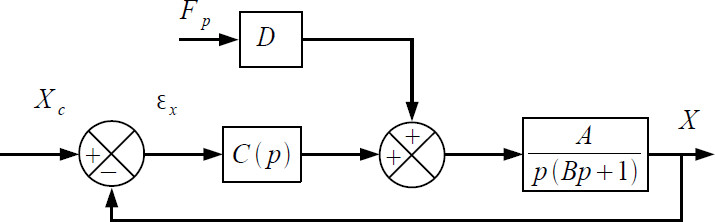
\includegraphics[width=\linewidth]{47_02}
%\caption{ \label{fig_47_02}}
\end{marginfigure}
\fi







\ifprof
\else

\marginnote{Corrigé voir \ref{B2:07:47}.}

\fi 
 
\graphicspath{{\repStyle/png/}{../SLCI/SLCI-03-SchemaBlocs/48_Quille/images/}} 
\normaltrue \difficilefalse \tdifficilefalse
\correctiontrue

%\UPSTIidClasse{11} % 11 sup, 12 spé
%\newcommand{\UPSTIidClasse}{11}

\exer{Quille pendulaire $\star$ \label{B2:07:48}}
\setcounter{question}{0}\marginnote{\xpComp{SLCI}{03}}%\UPSTIcompetence{B2-07}
\index{Compétence B2-07}\index{Compétence SLCI-03}
\index{Schéma-blocs}
\index{Fonctions de transfert}
\index{Quille pendulaire}
\ifcorrection
\else
\marginnote{\textbf{Pas de corrigé pour cet exercice.}}
\fi


\ifprof 
\else
Le comportement d'un vérin est défini par le modèle continu de la figure \ref{B2:07:48_fig1}.


\begin{figure}[!h]
\begin{tikzpicture}
\sbEntree{E}

\sbBloc[3]{b0}{$A_1$}{E}
    \sbRelier[$Q(p)$]{E}{b0}


\sbComp{c1}{b0}
    \sbRelier{b0}{c1}

\sbBloc[1]{b1}{$A_2$}{c1}
    \sbRelier{c1}{b1}
    
\sbBloc[3]{b11}{$A_3$}{b1}
    \sbRelier[$\Sigma(p)$]{b1}{b11}


\sbComph{c2}{b11}
    \sbRelier{b11}{c2}

\sbBloc{b2}{$A_4$}{c2}
    \sbRelier{c2}{b2}
    

\sbSortie[4]{S}{b2}
    \sbRelier{b2}{S}
    \sbNomLien[0.8]{S}{$X(p)$}
  
\sbRenvoi{b2-S}{c1}{}

\draw [latex-] (c2) --++ (0,1) node[left] {$F_R(p)$};

\end{tikzpicture}
\caption{Asservissement en débit du vérin \label{B2:07:48_fig1}}
\end{figure}


On a : 
\begin{itemize}
\item $q(t)=S\dfrac{\dd x(t)}{ \dd t}+\dfrac{V}{2B}\dfrac{\dd \sigma(t)}{\dd t}$ (a);
\item $M\dfrac{\dd^2 x(t)}{\dd t^2} = S \sigma(t) - kx(t)-\lambda \dfrac{\dd x(t)}{\dd t} - f_R(t)$ (b).
\end{itemize}

On a :
\begin{itemize}
\item $\mathcal{L}\left(q(t)\right)=Q(p)$ : débit d’alimentation du vérin $\left[\text{m}^3\text{s}^{-1}\right]$;
\item $\mathcal{L}\left(\sigma(t)\right)=\Sigma(p)$ : différence de pression entre les deux chambres du vérin $\left[\text{Pa}\right]$;
\item $\mathcal{L}\left(x(t)\right)=X(p)$ : position de la tige du vérin $\left[\text{m}\right]$;
\item $\mathcal{L}\left(f_R(t)\right)=F_R(p)$ : composante selon l'axe de la tige du vérin de la résultante du torseur d'inter-effort de la liaison pivot entre tige et quille $\left[\text{N}\right]$.
\end{itemize}
Les constantes sont les suivantes :
\begin{itemize}
\item $S$ : section du vérin $\left[\text{m}^2\right]$;
\item $k$ : raideur mécanique du vérin $\left[\text{N\,m}^{-1}\right]$;
\item $V$ : volume d'huile de référence $\left[\text{m}^{3}\right]$;
\item $B$ : coefficient de compressibilité de l'huile $\left[\text{N\, m}^{-2}\right]$;
\item $M$ : masse équivalente à l'ensemble des éléments mobiles ramenés sur la tige du vérin $\left[\text{kg}\right]$;
\item $\lambda$ : coefficient de frottement visqueux$\left[\text{N\,m}^{-1}\text{s}\right]$.
\end{itemize} 

\fi
\question{Donner les expressions des fonctions de transfert $A_1$, $A_2$, $A_3$ et $A_4$ en fonction de la variable
complexe $p$ et des constantes.}
\ifprof

D'une part, on transforme les équations dans le domaine de Laplace : 
$Q(p)=S p X(p)+\dfrac{V}{2B} p \Sigma(p)$ et
$Mp^2 X(p) = S \Sigma(p) - kX(p)-\lambda p X(p) - F_R(p)$.

En utilisant le schéma-blocs, on a $\Sigma(p)=A_2\left(A_1Q(p)-X(p)\right) = A_1A_2Q(p)-A_2X(p)$.

Par ailleurs $\Sigma(p)=\dfrac{Q(p)-S p X(p)}{\dfrac{V}{2B} p}= Q(p)\dfrac{2B}{Vp}-  X(p)  \dfrac{S2B}{V} $. On a donc $A_2 = \dfrac{S2B}{V} $, $A_1 A_2 = \dfrac{2B}{Vp}$ soit $A_1  = \dfrac{2B}{Vp}\dfrac{V}{S2B}= \dfrac{1}{Sp}$. 


On a aussi $X(p)=A_4\left(-F_R(p)+A_3\Sigma(p)\right) =-A_4F_R(p)+A_3A_4\Sigma(p)$. Par ailleurs,
$X(p) \left(Mp^2  +\lambda p  + k\right)= S \Sigma(p) - F_R(p) \Leftrightarrow X(p) =  \dfrac{S \Sigma(p)}{Mp^2  +\lambda p  + k}-\dfrac{F_R(p)}{Mp^2  +\lambda p  + k}$. On a donc : $A_4 = \dfrac{1}{Mp^2  +\lambda p  + k}$ et $A_3 = S$.

Au final,  $A_1=\dfrac{1}{Sp}$,  $A_2 = \dfrac{S2B}{V} $,  $A_3 = S$  et $A_4 = \dfrac{1}{Mp^2  +\lambda p  + k}$.

\else
\fi

\ifprof
\else

Le schéma-blocs de la figure précédente peut se mettre sous la forme de la figure \ref{B2:07:48_fig2}. 

\footnotesize
\begin{marginfigure}
\begin{tikzpicture}
\sbEntree{E}

\sbBloc[3]{b1}{$H_1$}{E}
    \sbRelier[$Q(p)$]{E}{b1}


\sbComph{c1}{b1}
    \sbRelier{b1}{c1}
  
\sbBloc{b2}{$H_2$}{c1}
    \sbRelier{c1}{b2}

\sbSortie{S}{b2}
    \sbRelier{b2}{S}
    \sbNomLien[0.8]{S}{$X(p)$}

%\sbBloc[3]{b11}{$A_3$}{b1}
%    \sbRelier[$\Sigma(p)$]{b1}{b11}
%
%
%\sbSumh{c2}{b11}
%    \sbRelier{b11}{c2}
%
%\sbBloc{b2}{$A_4$}{c2}
%    \sbRelier{c2}{b2}
%    
%
%\sbSortie[4]{S}{b2}
%    \sbRelier{b2}{S}
%    \sbNomLien[0.8]{S}{$X(p)$}
%  
%\sbRenvoi{b2-S}{c1}{}
%
\draw [latex-] (c1) --++ (0,1) node[left] {$F_R(p)$};

\end{tikzpicture}
\caption{Schéma-bloc \label{B2:07:48_fig2}}
\end{marginfigure}
\normalsize

\fi

\question{Donner les expressions des fonctions de transfert $H_1$
et $H_2$ en fonction de $A_1$, $A_2$, $A_3$ et $A_4$, puis de la variable $p$ et
des constantes.}
\ifprof

\textbf{Méthode 1 : Utilisation des relations précédentes}
On a $X(p)=\left(H_1Q(p)-F_R(p)\right)H_2(p)$. 

Par ailleurs, on a vu que $X(p)=A_4\left(-F_R(p)+A_3\Sigma(p)\right) $ et $\Sigma(p)=A_2\left(A_1Q(p)-X(p)\right)$. 

On a donc $X(p)=A_4\left(-F_R(p)+A_3  A_2\left(A_1Q(p)-X(p)\right)\right) $ $ \Leftrightarrow X(p)\left(1+A_2A_3A_4 \right)=A_4\left(-F_R(p)+A_3  A_2A_1Q(p)\right) $. On a donc 
$H_1(p)=A_1  A_2A_3$ et $H_2 = \dfrac{A_4}{1+ A_2A_3A_4 }$.

\textbf{Méthode 2 : Lecture directe du schéma-blocs}
Revient à utiliser la méthode précédente. 

\textbf{Méthode 3 : Algèbre de schéma-blocs}
Le schéma-blocs proposé est équivalent au schéma suivant. 

\footnotesize
\begin{figure}[!h]
\begin{tikzpicture}
\sbEntree{E}

\sbBloc[3]{b0}{$A_1 A_2 A_3$}{E}
    \sbRelier[$Q(p)$]{E}{b0}

\sbComph{c2}{b0}
    \sbRelier{b0}{c2}
    
\sbComp{c1}{c2}
    \sbRelier{c2}{c1}

\sbBloc{b1}{$A_4$}{c1}
    \sbRelier{c1}{b1}
    

\sbSortie[4]{S}{b1}
    \sbRelier{b1}{S}
    \sbNomLien[0.8]{S}{$X(p)$}
      
      
\sbDecaleNoeudy[4]{S}{U}
\sbDecaleNoeudx[-2]{U}{U2}
\sbBlocr{r1}{$A_2 A_3$}{U2}


\sbRelieryx{b1-S}{r1}
\sbRelierxy{r1}{c1}


%    
%\sbBloc[3]{b11}{$A_3$}{b1}
%    \sbRelier[$\Sigma(p)$]{b1}{b11}
%
%
%\sbComph{c2}{b11}
%    \sbRelier{b11}{c2}
%
%\sbBloc{b2}{$A_4$}{c2}
%    \sbRelier{c2}{b2}
%    
%
%\sbRenvoi{b2-S}{c1}{}

\draw [latex-] (c2) --++ (0,1) node[left] {$F_R(p)$};

\end{tikzpicture}
\end{figure}
\normalsize

On retrouve le même résultat que précédemment. 


$A_1=\dfrac{1}{Sp}$,  $A_2 = \dfrac{S2B}{V} $,  $A_3 = S$  et $A_4 = \dfrac{1}{Mp^2  +\lambda p  + k}$.


En faisant le calcul on obtient : 
$H_1(p)=\dfrac{2BS}{pV}  $ et $H_2 = \dfrac{\dfrac{1}{Mp^2  +\lambda p  + k}}{1+ \dfrac{2BS^2}{V}\dfrac{1}{Mp^2  +\lambda p  + k} }$  $= \dfrac{1}{Mp^2  +\lambda p  + k+ \dfrac{2BS^2}{V} }$.


\else
\fi

\question{Pour ce vérin non perturbé ($F_R=0$), donner sa fonction de transfert $X(p)/Q(p)$ en fonction de la variable $p$ et des constantes.}
\ifprof

Dans ce cas, $\dfrac{X(p)}{Q(p)}=H_1(p)H_2(p)=\dfrac{2BS}{p\left(MVp^2  +\lambda pV  + kV+ 2BS^2\right) }$.

\else
\fi








\ifprof
\else
\begin{solution}
\begin{enumerate}
\item $A_1=\dfrac{1}{Sp}$,  $A_2 = \dfrac{S2B}{V} $,  $A_3 = S$  et $A_4 = \dfrac{1}{Mp^2  +\lambda p  + k}$.
\item $H_1(p)=A_1  A_2A_3$ et $H_2 = \dfrac{A_4}{1+ A_2A_3A_4 }$.
\item $\dfrac{X(p)}{Q(p)}=\dfrac{2BS}{p\left(MVp^2  +\lambda pV  + kV+ 2BS^2\right) }$.
\end{enumerate} 
\end{solution}

\marginnote{Corrigé voir \ref{B2:07:47}.}

\fi 
 
\graphicspath{{\repStyle/png/}{../SLCI/SLCI-03-SchemaBlocs/500_Divers/images/}} 
\normaltrue \difficilefalse \tdifficilefalse
\correctiontrue

%\UPSTIidClasse{11} % 11 sup, 12 spé
%\newcommand{\UPSTIidClasse}{11}

\exer{Fonctions de transfert$\star$ \label{B2:07:500}}
\setcounter{question}{0}\marginnote{\xpComp{SLCI}{03}}%\UPSTIcompetence{B2-07}
\index{Compétence B2-07}\index{Compétence SLCI-03}
\index{Schéma-blocs}
\index{FTBO}
\index{FTBF}

\index{Forme canonique}
\ifcorrection
\else
\marginnote{\textbf{Pas de corrigé pour cet exercice.}}
\fi


\ifprof 
\else
Soit le schéma-blocs suivant.
\begin{marginfigure}
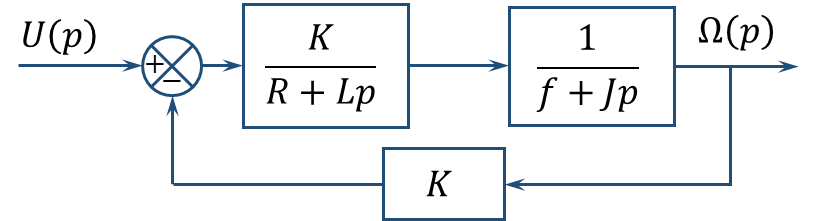
\includegraphics[width=\linewidth]{500_01}
\end{marginfigure}
 \fi
 
\question{Déterminer la fonction de transfert en boucle ouverte. Mettre l'expression sous forme canonique et exprimer les paramètres caractéristiques.}
\ifprof
On a $\text{FTBO}(p)=\dfrac{K^2}{\left(R+Lp\right)\left(f+Jp\right)}$
$=\dfrac{K^2}{Rf+RJp+Lfp+LJp^2}$
$=\dfrac{K^2}{Rf\left(1+p\dfrac{RJ+Lf}{Rf}+\dfrac{LJ}{Rf}p^2\right)}$.

On a donc $K_{\text{BO}}=\dfrac{K^2}{Rf}$, 
$\omega_{\text{BO}} = \sqrt{\dfrac{Rf}{LJ}}$,
$\dfrac{2\xi_{\text{BO}} }{\omega_{\text{BO}}}=\dfrac{RJ+Lf}{Rf} \Leftrightarrow
\xi_{\text{BO}} =\omega_{\text{BO}}\dfrac{RJ+Lf}{2Rf}
=\sqrt{\dfrac{Rf}{LJ}}\dfrac{RJ+Lf}{2Rf}
=\dfrac{RJ+Lf}{2\sqrt{LJRf}}$.
\else 
\fi

\question{Déterminer la fonction de transfert en boucle fermée. Mettre l'expression sous forme canonique et exprimer les paramètres caractéristiques.}
\ifprof
On a $\text{FTBF}(p)=\dfrac{\dfrac{K}{\left(R+Lp\right)\left(f+Jp\right)}}{1+\dfrac{K^2}{\left(R+Lp\right)\left(f+Jp\right)}}
=\dfrac{K}{\left(R+Lp\right)\left(f+Jp\right)+K^2}
=\dfrac{\dfrac{K}{K^2+Rf}}{\dfrac{RJ+Lf}{Rf+K^2}p+\dfrac{LJ}{Rf+K^2}p^2+1}$.



On a donc $K_{\text{BF}}=\dfrac{K}{K^2+Rf}$, 
$\omega_{\text{BF}} = \sqrt{\dfrac{Rf+K^2}{LJ}}$,
$\dfrac{2\xi_{\text{BF}} }{\omega_{\text{BF}}}=\dfrac{RJ+Lf}{Rf+K^2} \Leftrightarrow
\xi_{\text{BO}} =\omega_{\text{BF}}\dfrac{RJ+Lf}{2\left(Rf+K^2\right)}
=\sqrt{\dfrac{Rf+K^2}{LJ}}\dfrac{RJ+Lf}{2\left(Rf+K^2\right)}$
%=\sqrt{\dfrac{Rf}{LJ}}\dfrac{RJ+Lf}{2Rf}
%=\dfrac{RJ+Lf}{2\sqrt{LJRf}}$.
%
$\xi_{\text{BF}}=\dfrac{RJ+Lf}{2\sqrt{LJ}\sqrt{Rf+K^2}}$.
\else 
\fi

\ifprof 
\else
Soit le schéma-blocs suivant.
\begin{marginfigure}
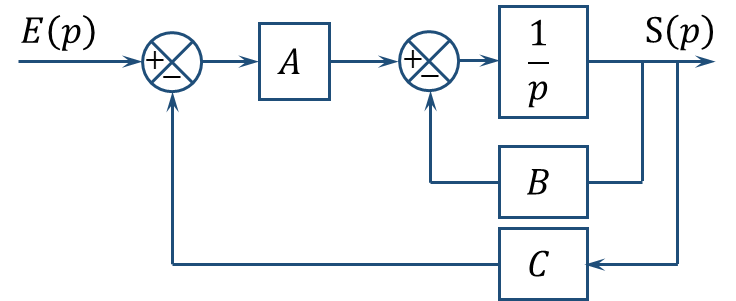
\includegraphics[width=\linewidth]{500_02}
\end{marginfigure}
 \fi
 
 \question{Déterminer la fonction de transfert en boucle ouverte. Mettre l'expression sous forme canonique et exprimer les paramétres caractéristiques.}
\ifprof
Si on note $R(p)$ la seconde entrée du \textbf{premier comparateur} et $\varepsilon(p)$ la sortie du premier comparateur,  

$\text{FTBO(p)}=\dfrac{\varepsilon(p)}{R(p)} = A \times \dfrac{\dfrac{1}{p}}{1+\dfrac{B}{p}}\times C = \dfrac{AC}{B+p} = \dfrac{\dfrac{AC}{B}}{1+\dfrac{p}{B}}$.
On a donc $K_{\text{BO}}=\dfrac{AC}{B}$ et $\tau_{\text{BO}}=\dfrac{1}{B}$.

\else 
\fi

 
\question{Déterminer la fonction de transfert en boucle fermée. Mettre l'expression sous forme canonique et exprimer les paramétres caractéristiques.}
\ifprof
On a
$\text{FTBF(p)} = \dfrac{\dfrac{A}{B+p}}{1+\dfrac{AC}{B+p}}=\dfrac{A}{B+p+AC}=\dfrac{\dfrac{A}{B+AC}}{1+\dfrac{p}{B+AC}}$.

On a donc $K_{\text{BF}}=\dfrac{A}{B+AC}$ et $\tau_{\text{BF}}=\dfrac{1}{B+AC}$.

\else 
\fi


%\question{Réaliser le schéma-blocs.}
%\ifprof
%\begin{marginfigure}
%\centering
%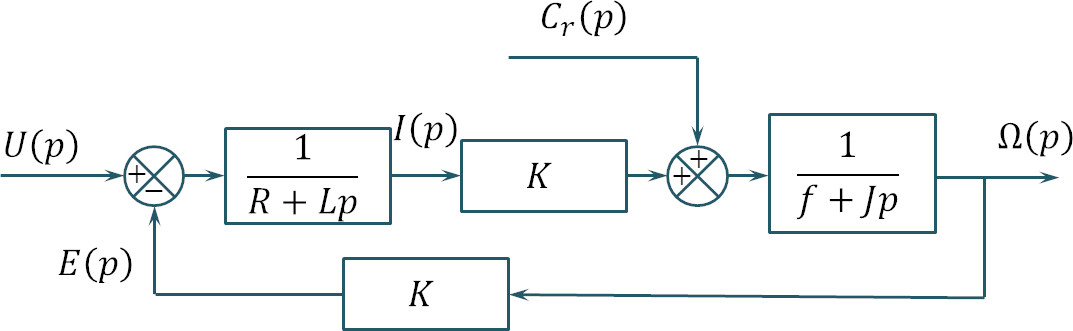
\includegraphics[width=\linewidth]{51_01_c}
%%\caption{Évolution du couple utile en fonction de la vitesse de rotation pour des
%%fréquences de commande de \SI{90}{Hz} à \SI{110}{Hz}. \label{fig_50_04}}
%\end{marginfigure}
%\else
%\fi


 

\ifprof
\else
\begin{solution}
\begin{enumerate}
\item $K_{\text{BO}}=\dfrac{K^2}{Rf}$, 
$\omega_{\text{BO}} = \sqrt{\dfrac{Rf}{LJ}}$,
$\xi_{\text{BO}} =\dfrac{RJ+Lf}{2\sqrt{LJRf}}$.
\item $K_{\text{BF}}=\dfrac{K}{K^2+Rf}$, 
$\xi_{\text{BF}}=\dfrac{RJ+Lf}{2\sqrt{LJ}\sqrt{Rf+K^2}}$.
\item $K_{\text{BO}}=\dfrac{AC}{B}$ et $\tau_{\text{BO}}=\dfrac{1}{B}$.
\item $K_{\text{BF}}=\dfrac{A}{B+AC}$ et $\tau_{\text{BF}}=\dfrac{1}{B+AC}$.
\end{enumerate}
\end{solution}
\marginnote{Corrigé voir \ref{B2:07:500}.}

\fi 
 
\graphicspath{{\repStyle/png/}{../SLCI/SLCI-03-SchemaBlocs/505_Divers/images/}} 
\normaltrue \difficilefalse \tdifficilefalse
\correctionfalse

%\UPSTIidClasse{11} % 11 sup, 12 spé
%\newcommand{\UPSTIidClasse}{11}

\exer{Calcul de FTBO$\star$ \label{B2:07:505}}
\setcounter{question}{0}\marginnote{\xpComp{SLCI}{03}}%\UPSTIcompetence{B2-07}
\index{Compétence B2-07}\index{Compétence SLCI-03}
\index{Schéma-blocs}
\index{FTBO}

\ifcorrection
\else
\marginnote{\textbf{Pas de corrigé pour cet exercice.}}
\fi


\question{Déterminer la FTBO dans la cas suivant.}

\ifprof 
$\text{FTBO}(p) = BCDE$.
\else
\begin{marginfigure}
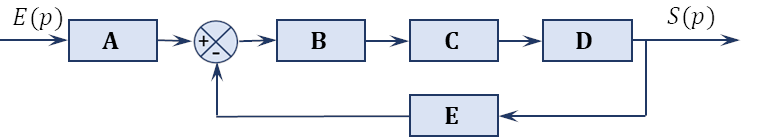
\includegraphics[width=\linewidth]{505_01}
\end{marginfigure}
\fi
 
\question{Déterminer la FTBO dans la cas suivant.}

\ifprof 
$\text{FTBO}(p) = B\left(1+A\right)$.
\else
\begin{marginfigure}
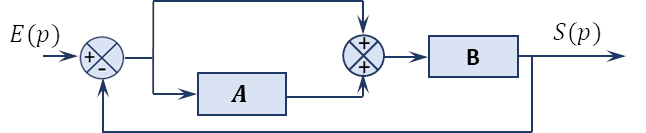
\includegraphics[width=\linewidth]{505_02}
\end{marginfigure}
\fi

\question{Déterminer la FTBO dans la cas suivant.}

\ifprof 
$\text{FTBO}(p) = A \dfrac{BCD}{1+BCD}$.
\else
\begin{marginfigure}
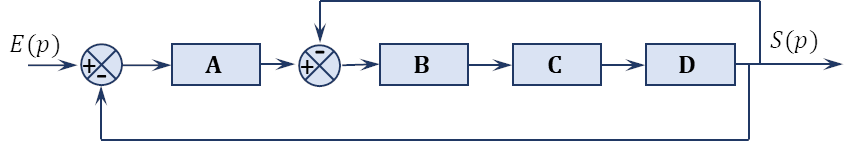
\includegraphics[width=\linewidth]{505_03}
\end{marginfigure}
\fi

\question{Déterminer la FTBO dans la cas suivant.}

\ifprof 
$\text{FTBO}(p) = A \dfrac{\dfrac{B}{1+B}CD}{1+\dfrac{B}{1+B}CD} = \dfrac{ABCD}{1+B+BCD}$.
\else
\begin{marginfigure}
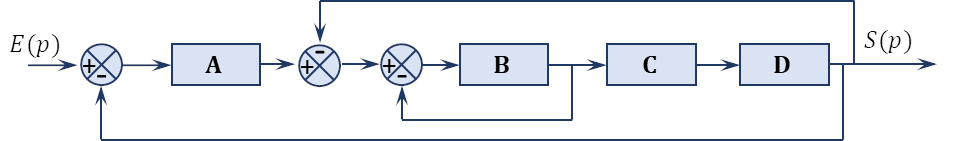
\includegraphics[width=\linewidth]{505_04}
\end{marginfigure}
\fi



%\question{Réaliser le schéma-blocs.}
%\ifprof
%\begin{marginfigure}
%\centering
%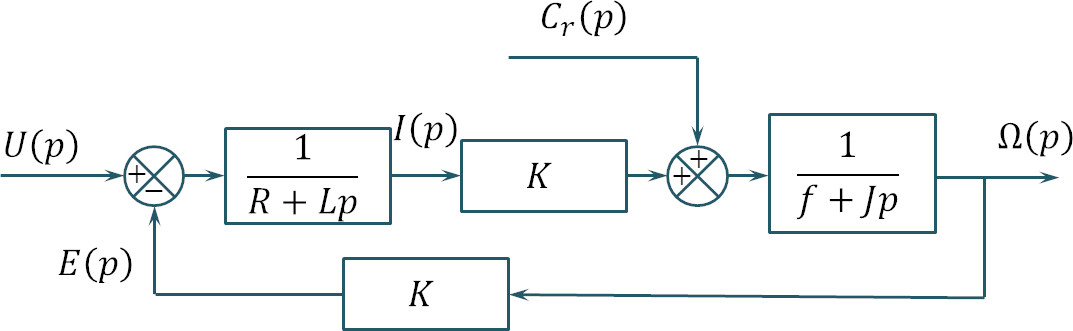
\includegraphics[width=\linewidth]{51_01_c}
%%\caption{Évolution du couple utile en fonction de la vitesse de rotation pour des
%%fréquences de commande de \SI{90}{Hz} à \SI{110}{Hz}. \label{fig_50_04}}
%\end{marginfigure}
%\else
%\fi


 

\ifprof
\else
\begin{solution}
\begin{enumerate}
\item $\text{FTBO}(p) = BCDE$.
\item $\text{FTBO}(p) = B\left(1+A\right)$.
\item $\text{FTBO}(p) = A \dfrac{BCD}{1+BCD}$.
\item $\text{FTBO}(p) = \dfrac{ABCD}{1+B+BCD}$.
\end{enumerate}
\end{solution}

\marginnote{Corrigé voir \ref{B2:07:505}.}

\fi 
 
\graphicspath{{\repStyle/png/}{../SLCI/SLCI-03-SchemaBlocs/512_Divers/images/}} 
\normaltrue \difficilefalse \tdifficilefalse
\correctionfalse

%\UPSTIidClasse{11} % 11 sup, 12 spé
%\newcommand{\UPSTIidClasse}{11}

\exer{Calcul de FTBO$\star$ \label{B2:07:505}}
\setcounter{question}{0}\UPSTIcompetence[2]{B2-07}
\index{Compétence B2-07}
\index{Schéma-blocs}
\index{FTBO}

\ifcorrection
\else
\marginnote{\textbf{Pas de corrigé pour cet exercice.}}
\fi


\question{Déterminer la FTBO dans la cas suivant.}
\ifprof 
\else
\begin{center}
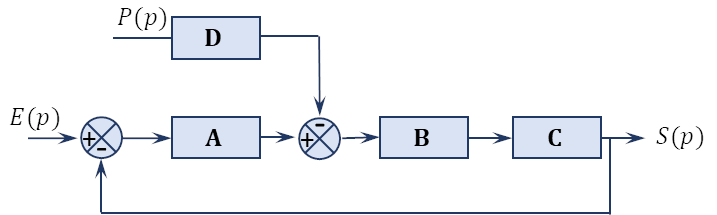
\includegraphics[width=.9\linewidth]{512_01}
\end{center}
\fi
 
\question{Déterminer la FTBO dans la cas suivant.}
\ifprof 
\else
\begin{center}
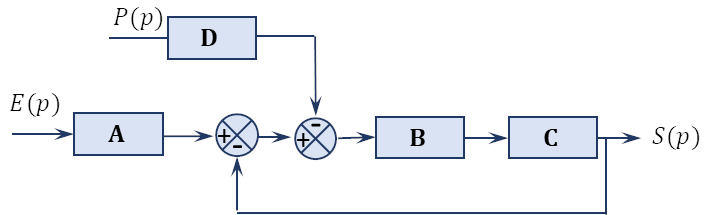
\includegraphics[width=.9\linewidth]{512_02}
\end{center}
\fi

\question{Déterminer la FTBO dans la cas suivant.}
\ifprof 
\else
\begin{center}
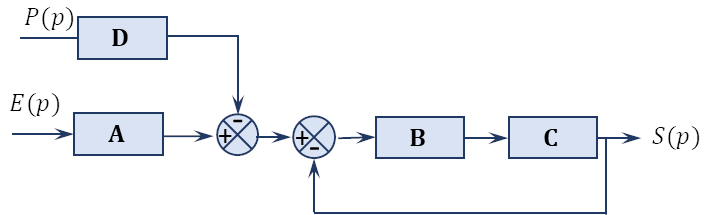
\includegraphics[width=.9\linewidth]{512_03}
\end{center}
\fi

\question{Déterminer la FTBO dans la cas suivant.}
\ifprof 
\else
\begin{center}
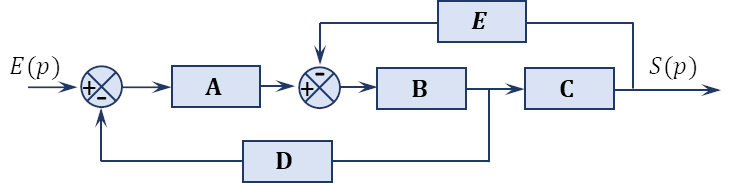
\includegraphics[width=.9\linewidth]{512_04}
\end{center}
\fi



%\question{Réaliser le schéma-blocs.}
%\ifprof
%\begin{figure}[H]
%\centering
%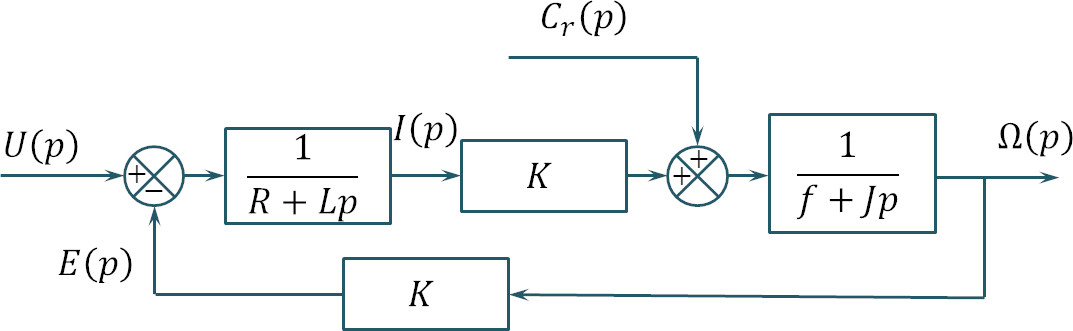
\includegraphics[width=\linewidth]{51_01_c}
%%\caption{Évolution du couple utile en fonction de la vitesse de rotation pour des
%%fréquences de commande de \SI{90}{Hz} à \SI{110}{Hz}. \label{fig_50_04}}
%\end{figure}
%\else
%\fi


 

\ifprof
\else
\begin{flushright}
\footnotesize{Corrigé  voir \ref{B2:07:505}.}
\end{flushright}%
\fi 
 
\graphicspath{{\repStyle/png/}{../SLCI/SLCI-03-SchemaBlocs/51_MCC/images/}} 
\normaltrue \difficilefalse \tdifficilefalse
\correctiontrue

%\UPSTIidClasse{11} % 11 sup, 12 spé
%\newcommand{\UPSTIidClasse}{11}

\exer{Moteur à courant continu$\star$ \label{B2:07:51}}
\setcounter{question}{0}\UPSTIcompetence[2]{B2-07}
\index{Compétence B2-07}
\index{Schéma-blocs}
\index{Moteur à courant continu}
\index{MCC}
\ifcorrection
\else
\marginnote{\textbf{Pas de corrigé pour cet exercice.}}
\fi


\ifprof 
\else
On donne les équations du moteur à courant continu :
\begin{itemize}
\item $u(t) = e(t)+ Ri(t) +L \dfrac{\text{d}i(t)}{\text{d} t}$;
\item $e(t)=K\omega(t)$;
\item $c(t)=Ki(t)$;
\item $c(t)+c_r(t)- f\omega(t)=J\dfrac{\text{d}\omega(t)}{\text{d} t}$.
\end{itemize}
\fi

\question{Réaliser le schéma-blocs.}
\ifprof
\begin{figure}[H]
\centering
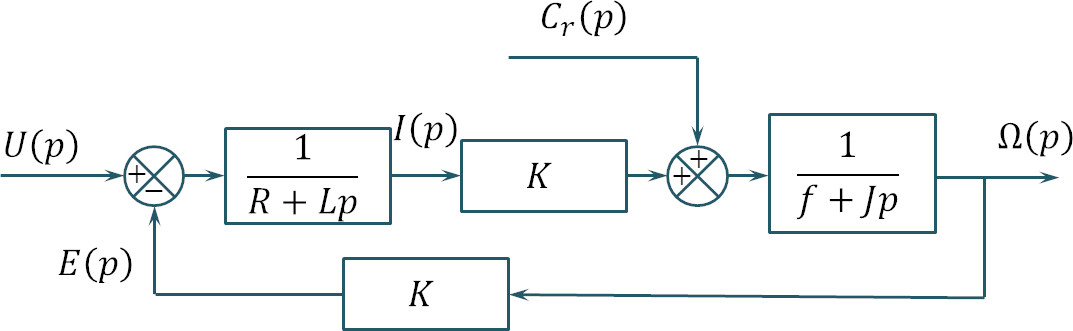
\includegraphics[width=.7\linewidth]{51_01_c}
%\caption{Évolution du couple utile en fonction de la vitesse de rotation pour des
%fréquences de commande de \SI{90}{Hz} à \SI{110}{Hz}. \label{fig_50_04}}
\end{figure}
\else
\fi



\question{Mettre le schéma-blocs sous la forme suivante.}
\ifprof
\begin{figure}[H]
\centering
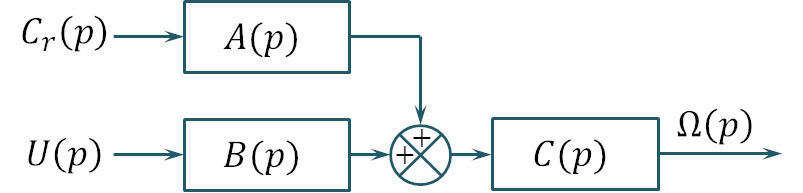
\includegraphics[width=.7\linewidth]{51_01}
%\caption{Évolution du couple utile en fonction de la vitesse de rotation pour des
%fréquences de commande de \SI{90}{Hz} à \SI{110}{Hz}. \label{fig_50_04}}
\end{figure}


En utilisant le schéma-blocs proposé, on a $\Omega(p) = \left(C_r(p)A(p)+U(p)B(p)\right)C(p)$.

D'autre part,  $\Omega(p)=\left( C_r(p) + \dfrac{K}{R+Lp}\left(U(p)-K\Omega(p) \right) \right) \dfrac{1}{f+Jp}$.

On a donc $\left(f+Jp \right)\Omega(p)= C_r(p) + U(p)\dfrac{K}{R+Lp}  $

$\Leftrightarrow \left(f+Jp \right)\Omega(p)+ \dfrac{K^2}{R+Lp}\Omega(p)  = C_r(p) + U(p)\dfrac{K}{R+Lp} $

$\Leftrightarrow \left(\left(f+Jp \right)+ \dfrac{K^2}{R+Lp}\right)\Omega(p)  = C_r(p) + U(p)\dfrac{K}{R+Lp} $

$\Leftrightarrow \dfrac{K^2+\left(f+Jp \right)\left(R+Lp \right)}{R+Lp}\Omega(p)  = C_r(p) + U(p)\dfrac{K}{R+Lp} $

$\Leftrightarrow \Omega(p)  = \left(C_r(p) + U(p)\dfrac{K}{R+Lp}\right)\dfrac{R+Lp}{K^2+\left(f+Jp \right)\left(R+Lp \right)} $.

Dés lors plusieurs schéma-blocs peuvent répondre à la question. Par exemple, $A(p)=1$, $B(p)=\dfrac{K}{R+Lp}$, $C(p)=\dfrac{R+Lp}{K^2+\left(f+Jp \right)\left(R+Lp \right)}$.

En poursuivant, on a aussi : 
$ \Omega(p)  = \left(C_r(p)(R+Lp) + U(p) K\right)\dfrac{1}{K^2+\left(f+Jp \right)\left(R+Lp \right)} $.

On a donc aussi,  $A(p)=R+Lp$, $B(p)={K}$, $C(p)=\dfrac{1}{K^2+\left(f+Jp \right)\left(R+Lp \right)}$



\else
\begin{figure}[H]
\centering
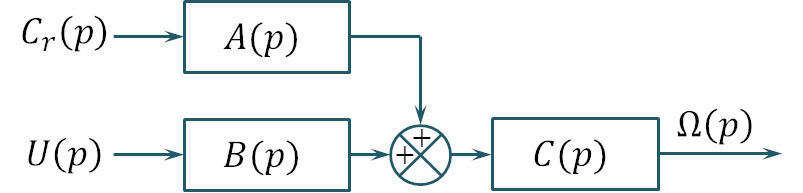
\includegraphics[width=.7\linewidth]{51_01}
%\caption{Évolution du couple utile en fonction de la vitesse de rotation pour des
%fréquences de commande de \SI{90}{Hz} à \SI{110}{Hz}. \label{fig_50_04}}
\end{figure}
\fi





\ifprof
\else

\ifcolle
\else
\noindent\footnotesize
\fbox{\parbox{.9\linewidth}{
Éléments de corrigé : 
\begin{enumerate}
    \item .
    \item $A(p)=R+Lp$, $B(p)={K}$, $C(p)=\dfrac{1}{K^2+\left(f+Jp \right)\left(R+Lp \right)}$ (plusieurs réponses possibles). 
\end{enumerate}}}
\normalsize
\fi
\begin{flushright}
\footnotesize{Corrigé  voir \ref{B2:07:51}.}
\end{flushright}%
\fi 
 
\graphicspath{{\repStyle/png/}{../SLCI/SLCI-03-SchemaBlocs/52_Verin/images/}} 
\normaltrue \difficilefalse \tdifficilefalse
\correctionfalse

%\UPSTIidClasse{11} % 11 sup, 12 spé
%\newcommand{\UPSTIidClasse}{11}

\exer{Vérin$\star$ \label{B2:07:52}}
\setcounter{question}{0}\marginnote{\xpComp{SLCI}{03}}%\UPSTIcompetence{B2-07}
\index{Compétence B2-07}\index{Compétence SLCI-03}
\index{Schéma-blocs}
\index{Vérin}
\ifcorrection
\else
\marginnote{\textbf{Pas de corrigé pour cet exercice.}}
\fi


\ifprof 
\else
On donne le schéma de principe d'une servo-commande.
\begin{marginfigure}
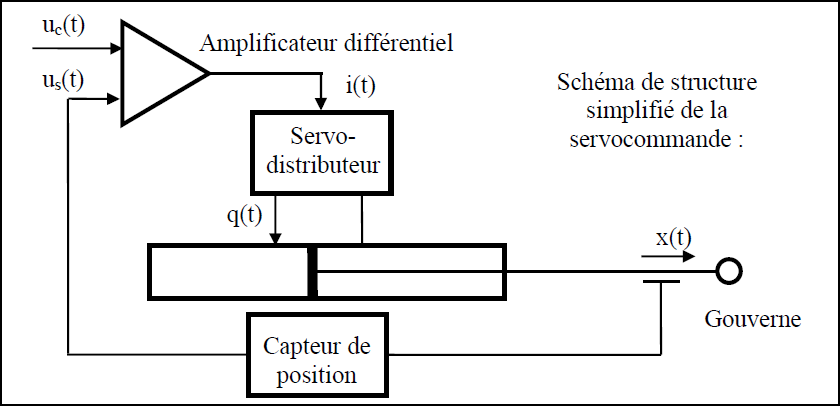
\includegraphics[width=\linewidth]{52_01}
\end{marginfigure}

Les différentes équations temporelles qui modélisent le fonctionnement d'une servocommande sont :
\begin{itemize}
\item un amplificateur différentiel défini par : $u_c(t)=\dfrac{i(t)}{K_a}+u_s(t)$;
\item débit dans le vérin dans le cas d'une hypothèse de fluide incompressible $q(t)=S\cdot\dfrac{\dd x(t)}{\dd t}$;
\item capteur de position : $u_s(t)=K_c\cdot x(t)$;
\item le servo-distributeur est un composant de la chaîne de commande conçu pour fournir un débit hydraulique $q(t)$ proportionnel au courant de commande $i(t)$. (Attention, valable uniquement en régime permanent.) On a 
$q(t)+T \dfrac{\dd q(t)}{\dd t} = K_d i(t)$.
%Le constructeur fournit sa fonction de transfert :
%$$
%F(p)=\dfrac{Q(p)}{I(p)}=\dfrac{K_d}{1+Tp}
%$$
%où $K_d$ est le gain du servo-distributeur et $T$ sa constante de temps.
\end{itemize}
 \fi
 
\question{Réaliser le schéma-blocs.}

\ifprof
On a :
\begin{itemize}
\item $U_c(p)=\dfrac{1}{K_a}I(p)+U_s(p)$
\item $Q(p)=SpX(p)$
\item $U_S(p)=K_C\cdot X(p)$
\item $F(p)=\dfrac{Q(p)}{I(p)}=\dfrac{K_d}{1+Tp}$
\end{itemize}

%\begin{minipage}[c]{.23\linewidth}
%\begin{marginfigure}
%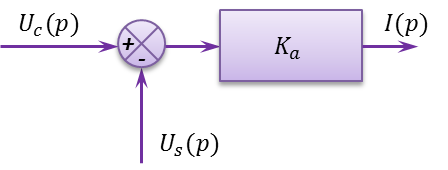
\includegraphics[width=.95\textwidth]{bloc1}
%\end{marginfigure}
%\end{minipage}\hfill
%\begin{minipage}[c]{.23\linewidth}
%\begin{marginfigure}
%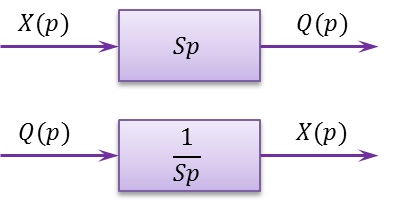
\includegraphics[width=.95\textwidth]{bloc2}
%\end{marginfigure}
%\end{minipage}\hfill
%\begin{minipage}[c]{.23\linewidth}
%\begin{marginfigure}
%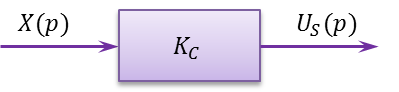
\includegraphics[width=.95\textwidth]{bloc3}
%\end{marginfigure}
%\end{minipage}\hfill
%\begin{minipage}[c]{.23\linewidth}
%\begin{marginfigure}
%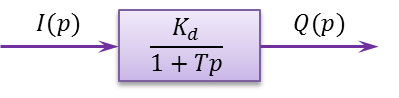
\includegraphics[width=.95\textwidth]{bloc4}
%\end{marginfigure}
%\end{minipage}

\begin{marginfigure}
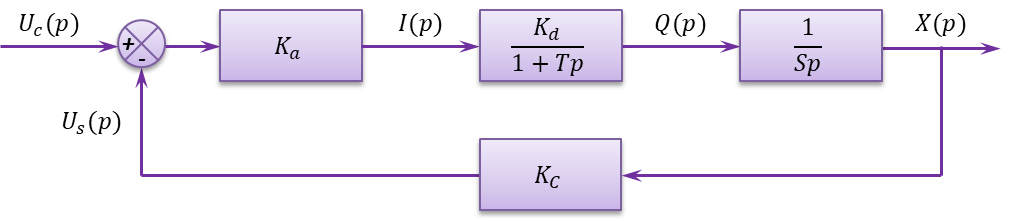
\includegraphics[width=\linewidth]{cor_01}
\end{marginfigure}

\else 
\fi


%\question{Réaliser le schéma-blocs.}
%\ifprof
%\begin{marginfigure}
%\centering
%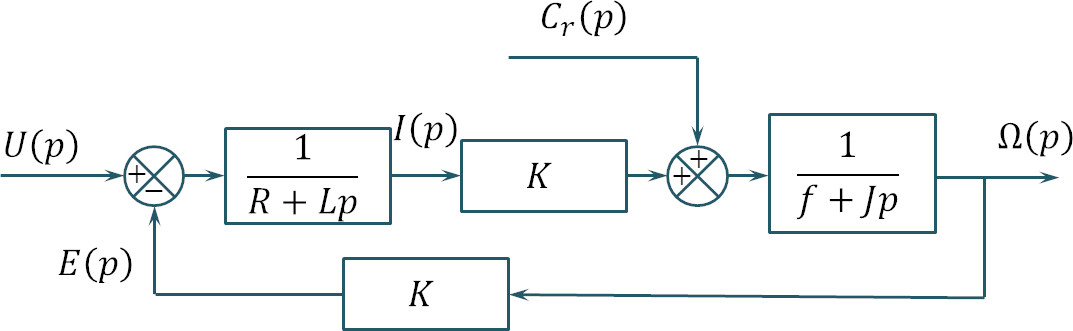
\includegraphics[width=\linewidth]{51_01_c}
%%\caption{Évolution du couple utile en fonction de la vitesse de rotation pour des
%%fréquences de commande de \SI{90}{Hz} à \SI{110}{Hz}. \label{fig_50_04}}
%\end{marginfigure}
%\else
%\fi


 

\ifprof
\else

\marginnote{Corrigé voir \ref{B2:07:52}.}

\fi 
 
\graphicspath{{\repStyle/png/}{../SLCI/SLCI-03-SchemaBlocs/53_BancEpreuveHydraulique/images/}} 
\normalfalse \difficiletrue \tdifficilefalse
\correctionfalse

%\UPSTIidClasse{11} % 11 sup, 12 spé
%\newcommand{\UPSTIidClasse}{11}

\exer{Banc d'épreuve hydraulique $\star$ \label{B2:07:53}}
\setcounter{question}{0}\UPSTIcompetence[2]{B2-07}
\index{Compétence B2-07}
\index{Schéma-blocs}
\index{Banc d'épreuve hydraulique}
\ifcorrection
\else
\marginnote{\textbf{Pas de corrigé pour cet exercice.}}
\fi

\ifprof
\else

\subsubsection*{Analyse de la fonction technique << mettre le tube sous pression >>.}

Un schéma hydraulique simplifié est donné figure suivante.
\begin{center}
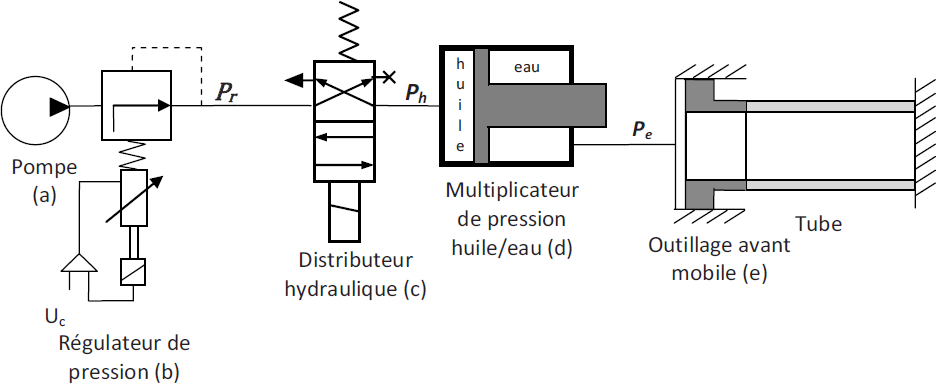
\includegraphics[width=\linewidth]{fig_01}

\end{center}


\subsubsection*{Mise en place du modèle}

Les équations du débit sont : 
$$Q_e(t)=S_e\dfrac{\dd z(t)}{\dd t} - \dfrac{V_{e0}}{B_e}\dfrac{\dd P_e(t)}{\dd t}$$ et 
$$Q_h(t)=S_h\dfrac{\dd z(t)}{\dd t} + \dfrac{V_{h0}}{B_h}\dfrac{\dd P_h(t)}{\dd t}.$$

En appliquant le théorème de la résultante dynamique selon $\vect{z}$ sur le piston du multiplicateur, on a : 
$
M\ddot{z}(t)=S_hp_h(t)-S_ep_e(t)-Mg-f\dot{z}(t).
$

\fi
\question{Déduire de la relation précédente l’équation reliant $Z(p)$, $P_e(p)$, $P_h(p)$, et $\text{Poids}(p)=Mg/p$, transformées de Laplace de $z(t)$, $P_e(t)$, $P_h(t)$ et du poids perçu comme une perturbation. Les conditions initiales sont supposées nulles.}
\ifprof

$Mp^2 Z(p))=S_hP_h(p)-S_eP_e(pt)-\dfrac{Mg}{p}-fpZ(p)$

\else
\fi


\ifprof
\else
On note :
\begin{itemize}
	\item $L(t)$ la position de l’équipage mobile repérée par rapport à sa position initiale;
	\item $V_t(t)$ le volume du tube;
	\item $F_t(t)$ l’effort du tube sur l’équipage mobile, avec $F_t(t) = - rL(t)$.
\end{itemize}

On néglige les variations de volume du tube dues à ses déformations. L’équation du débit s’écrit alors :
	$$Q_e (t)=(S_a-S_b ).\dfrac{\text{d}L(t)}{\text{d}t}+\dfrac{V_t}{B_e}  \dfrac{\text{d}P_e (t)}{\text{d}t}.$$

L’équation du mouvement de l’équipage mobile est donnée par : 
$$
m\ddot{L}(t)=-rL(t)+\left(S_a-S_b \right)p_e(t)-f'\dot{L}(t).
$$
\fi

\question{En déduire, en tenant compte de l’équation du débit, deux équations liant $L(p)$, $P_e(p)$ et $Q_e(p)$, transformées de Laplace de $L(t)$, $P_e(t)$ et $Q_e(t)$. Les conditions initiales sont supposées nulles.}
\ifprof

$Q_e (p)=(S_a-S_b )p L(p)+\dfrac{V_t}{B_e}  p P_e(p)$ et 
$mp^2{L}(p)=-rL(p)+\left(S_a-S_b \right)P_e(p)-f'p{L}(p)$.

\else

\fi

\question{Compléter le schéma-blocs de l’ensemble (sans le distributeur hydraulique), l’entrée étant la pression d’huile régulée $P_r(p)$ et la sortie la pression d’épreuve dans le tube $P_e(p)$.}
\ifprof

\else
\fi

\ifprof
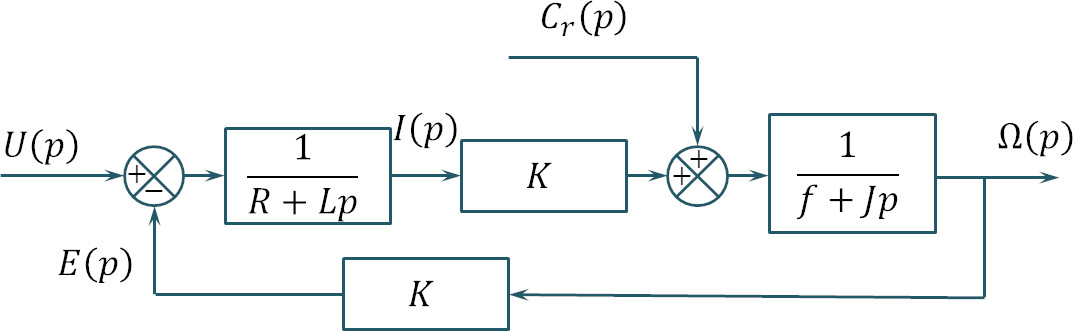
\includegraphics[width=\linewidth]{cor_01}
\else
\begin{center}
\rotatebox{90}{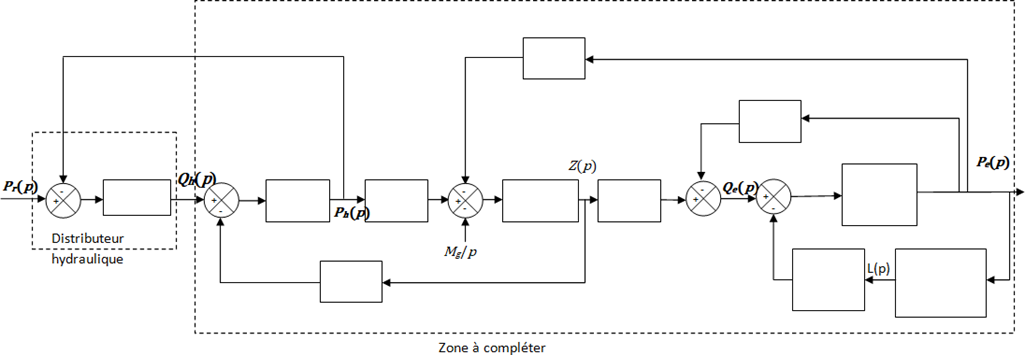
\includegraphics[height=.8\linewidth]{fig_10}}
\end{center}
\fi
 

\ifprof
\else
\begin{flushright}
\footnotesize{Corrigé  voir \ref{B2:07:52}.}
\end{flushright}%
\fi 
 
\graphicspath{{\repStyle/png/}{../SLCI/SLCI-03-SchemaBlocs/71_Robovolc/images/}} 
\normalfalse \difficiletrue \tdifficilefalse
\correctiontrue

%\UPSTIidClasse{11} % 11 sup, 12 spé
%\newcommand{\UPSTIidClasse}{11}

\exer{Robovolc $\star$ \label{B2:07:71}}
\setcounter{question}{0}\marginnote{\xpComp{SLCI}{03}}%\UPSTIcompetence{B2-07}
\index{Compétence B2-07}\index{Compétence SLCI-03}
\index{Schéma-blocs}
\index{Robovolc}
\ifcorrection
\else
\marginnote{\textbf{Pas de corrigé pour cet exercice.}}
\fi

\ifprof
\else

On considère le schéma-blocs suivant.
\begin{figure}[!h]
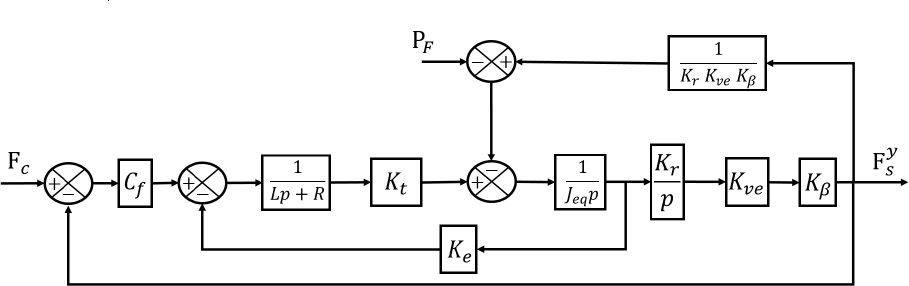
\includegraphics[width=9cm]{71_01}
\end{figure}
\fi
\question{En considérant $P_F=0$ (perturbation nulle) et $L=0$ (inductance nulle), calculer la fonction de transfert
$\dfrac{F_S^y}{F_c}$ et la mettre sous la forme canonique $\dfrac{K}{1+Ap+Bp^2}$. Identifier les paramètres $K$,
$A$ et $B$.}
\ifprof
\begin{corrige}

$\dfrac{F_S^y (p)}{F_C (p)}=\dfrac{C_f K_t K_r K_{ve} K_{\beta}}{R+C_f K_t K_r K_{ve} K_{\beta} } \times \dfrac{1}{1+\dfrac{K_e K_t}{R+C_f K_t K_r K_{ve} K_{\beta} }p+\dfrac{RJ_{eq}}{R+C_f K_t K_r K_{ve} K_{\beta} } p^2}$.


Par identification, on obtient :
$K=\dfrac{C_f K_t K_r K_{ve} K_{\beta}}{R+C_f K_t K_r K_{ve} K_{\beta}}$
$A=\dfrac{K_e K_t}{R+C_f K_t K_r K_{ve} K_{\beta} }$;
$B=\dfrac{RJ_{\text{eq}}}{R+C_f K_t K_r K_ve K_{\beta} }$.

\end{corrige}
\else
\fi

 
 \ifprof
\else
\ifcolle
\else
\footnotesize
\begin{solution}
\begin{enumerate}
\item $K=\dfrac{C_f K_t K_r K_{ve} K_{\beta}}{R+C_f K_t K_r K_{ve} K_{\beta}}$,
$A=\dfrac{K_e K_t}{R+C_f K_t K_r K_{ve} K_{\beta} }$,
$B=\dfrac{RJ_{\text{eq}}}{R+C_f K_t K_r K_ve K_{\beta} }$.
\end{enumerate} 
\end{solution}
\fi

\fi


\ifprof
\else

\marginnote{Corrigé voir \ref{B2:07:71}.}

\fi 
 
\graphicspath{{\repStyle/png/}{../SLCI/SLCI-03-SchemaBlocs/77_ProtheseTibia/images/}} 
\normaltrue \difficilefalse \tdifficilefalse
\correctiontrue

%\UPSTIidClasse{11} % 11 sup, 12 spé
%\newcommand{\UPSTIidClasse}{11}

\exer{Prothèse active transtibiale$\star$ \label{B2:07:77}}

% Concours Mines Ponts MP -- PSI --  2013

\setcounter{question}{0}\marginnote{\xpComp{SLCI}{03}}%\UPSTIcompetence{B2-07}
\index{Compétence B2-07}\index{Compétence SLCI-03}\index{Compétence SLCI-03}
\index{Schéma-blocs}
\index{Prothèse}
\ifcorrection
\else
\marginnote{\textbf{Pas de corrigé pour cet exercice.}}
\fi




\subsection*{Présentation}
%La majorité des prothèses transtibiales (pour une
%amputation en dessous du genou) utilisées aujourd'hui
%sont purement passives, c'est-à-dire que leurs
%propriétés mécaniques restent fixes pendant la marche.
%Ces prothèses sont constituées en général de semelles
%ressorts en carbone profilées qui emmagasinent et
%restituent l'énergie mécanique pendant la marche par
%déformation.

%\noindent\begin{minipage}[c]{.55\linewidth}
\ifprof
\else
Des ingénieurs du M.I.T. ont mis au point une prothèse active transtibiale capable de proposer un comportement
similaire à celui des membres non amputés. On étudie dans ce sujet le prototype initial
qui a permis de valider la pertinence d'une telle prothèse active.

%\end{minipage} \hfill
%\begin{minipage}[c]{.2\linewidth}
%\begin{marginfigure}
%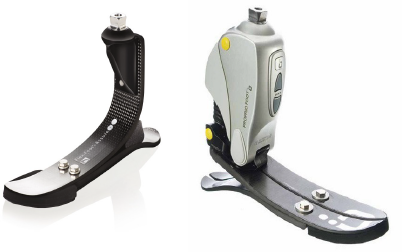
\includegraphics[height=2cm]{images/ccmp_01}

%\textit{Prothèse passive}
%\end{marginfigure}
%\end{minipage} \hfill
%\begin{minipage}[c]{.2\linewidth}
\begin{marginfigure}
\includegraphics[width=\linewidth]{ccmp_05}
\caption{Prothèse active}
\end{marginfigure}
%\end{minipage} 



%\noindent\begin{minipage}[c]{.65\linewidth}
L'actionneur de la prothèse est un moteur à courant continu alimenté par une batterie rechargeable de \SI{16}{V}. L'énergie mécanique est transmise par un
réducteur de type poulies-courroie suivi d'un
système vis-écrou qui adapte cette énergie
mécanique pour la prothèse (ensemble de liaisons
entre le pied artificiel constitué d'une semelle en
fibres de carbone et le manchon ou tibia artificiel).
Des ressorts permettent d'ajuster également l'énergie
mécanique fournie au pied artificiel. L'effort exercé
par les ressorts est directement relié au couple
exercé par l'actionneur.

%La chaîne d'informations est constituée d'un
%ensemble de capteurs permettant d'acquérir
%différentes informations :
%\begin{itemize}
%\item un potentiomètre linéaire qui mesure
%l'allongement/écrasement du ressort;
%\item un codeur incrémental placé au niveau de
%l'articulation pied/tibia;
%\item plusieurs capteurs capacitifs disposés sous
%la semelle du pied au niveau du talon et
%à l'avant du pied.
%\end{itemize}
%\end{minipage} \hfill
%\begin{minipage}[c]{.3\linewidth}
%\begin{marginfigure}
%\includegraphics[width=\linewidth]{images/ccmp_05}
%\textit{Prothèse passive}
%\end{marginfigure}
%\end{minipage}


On peut modéliser la chaîne d'énergie de la façon suivante : 
\begin{figure}[!h]
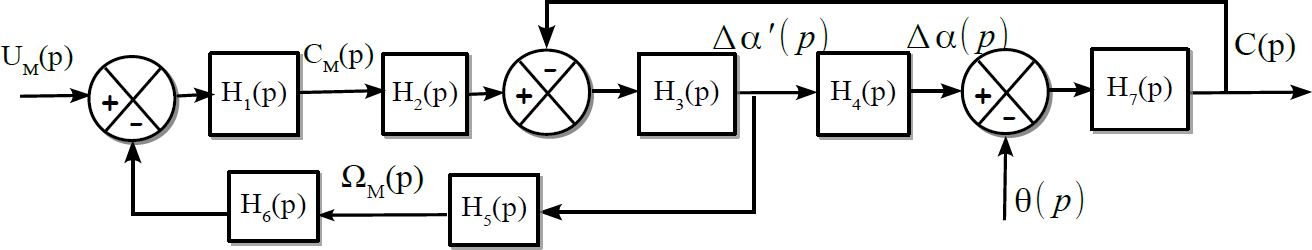
\includegraphics[width=\linewidth]{ccmp_07}
\end{figure}

Les grandeurs temporelles sont les suivantes :
\begin{itemize}
\item $u_M$ tension d'alimentation du moteur (V);
\item $C_M$ couple exercé par le moteur (Nm);
\item $\omega_M$ vitesse angulaire du moteur (rad\, $\text{s}^{-1}$);
\item $\alpha$ angle de rotation du basculeur (rad) tel que $\alpha=\alpha_r+\Delta \alpha$ où $\alpha_r$ est la position repos et $\Delta \alpha$  est la variation angulaire autour de la position repos. On a alors : $\dfrac{\dd \alpha}{\dd t}=\dfrac{\dd \Delta \alpha}{\dd t}$. On note $\Delta \alpha' ( p)$ la transformée de Laplace de $\dfrac{\dd \Delta \alpha}{\dd t}$;
\item $\theta$ angle de rotation du pied (rad) tel que $\theta = \SI{0}{rad}$ pour la position repos;
\item $C$ couple exercé par le pied (Nm).
\end{itemize}
On note en majuscule, lorsque cela est possible, les variables associées aux grandeurs temporelles dans le
domaine symbolique.
%
%\subsection{Modélisation de la chaîne de transmission}
%\begin{obj}
%L'objectif de cette partie est de valider l'aptitude du système à reproduire un mouvement du pied à la
%vitesse angulaire maximale de \SI{5,2}{rad.s^{-1}} spécifiée dans le cahier des charges. Dans un premier temps, il
%s'agira de déterminer la relation entre la rotation du pied artificiel par rapport au tibia et la translation de la tige
%du vérin électrique. Dans un second temps, une analyse plus fine du fonctionnement du vérin électrique permettra
%de remonter à la vitesse angulaire du moteur.
%\end{obj}
%
%La vitesse angulaire maximale est atteinte durant la
%phase oscillante (le pied n'est plus en contact avec le
%sol). Durant cette phase, nous supposerons que le pied
%et le basculeur ne possèdent pas de mouvement relatif.
%Rechercher une relation entre $\theta$ et $\lambda$, revient donc à
%déterminer la relation entre $\alpha$ et $\lambda$.
%
%
%Le vérin électrique est mis en mouvement par l'intermédiaire d'un moteur électrique à courant continu. Le mouvement de rotation du moteur est adapté par l'intermédiaire d'un système poulies-courroie suivi d'un système vis-écrou. On note $\omega_M$ la vitesse angulaire du rotor du moteur par rapport au stator.
%
%\begin{marginfigure}
%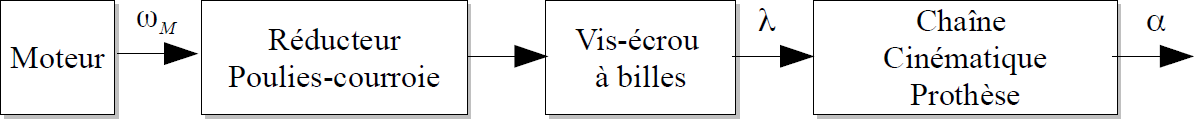
\includegraphics[width=\linewidth]{images/ccmp_08}
%\end{marginfigure}
%
%Le système vis-écrou est équipé d'une vis à billes de pas à droite $p_v$ avec $p_v=\SI{3}{mm.tour^{-1}}$. Le réducteur poulie-courroie possède un rapport de réduction $k=\dfrac{1}{2,1}$. On note $R_T$ le rapport entre la vitesse angulaire du rotor du moteur $\omega_M$ et la vitesse angulaire $\dfrac{\dd \alpha}{\dd t}$ tel que $\dfrac{\dd \alpha}{\dd t}=R_T\omega_M$.
%
%\question{En déduire les expressions littérales des blocs $H_4( p)$ et $H_5( p)$ . Déterminer la valeur numérique de $R_T$ . Conclure sur l'aptitude du moteur à générer la vitesse maximale exigée.}
\fi

\subsection*{Comportement dynamique de la prothèse}
\ifprof
\else
\begin{obj}
L'objectif de cette partie est d'établir les équations de comportement dynamique de la prothèse autour de
la position de repos lors des phases d'appui et oscillante. Ces équations permettront de compléter le schéma-blocs
de la chaîne d'énergie.
\end{obj}


On donne l'équation différentielle linéarisée suivante qui caractérise le comportement dynamique de la prothèse :
$
J_M \dfrac{\dd^2 \Delta \alpha(t) }{\dd t^2} + \mu_m \dfrac{\dd \Delta \alpha(t) }{\dd t} = C_M(t)R_T -C(t)R_T^2$  avec  $R_T = \dfrac{1}{145}$.

Le moteur électrique est régi par les équations électriques et de couplage électromécanique :
\begin{itemize}
\item $u_M (t )=Ri (t)+e(t)$ avec $i (t )$ courant moteur et $e(t )$ fcem;
\item $e (t )=k_c \omega_M (t )$ avec $\omega_M (t )$ vitesse angulaire du rotor du moteur par rapport au stator;
\item $C_M (t )=k_c i (t )$.
\end{itemize}


%Les constantes intervenant dans ces équations sont définies dans le tableau suivant.
%
%
%\begin{marginfigure}
%\begin{tabular}{|p{.45\linewidth}|p{.45\linewidth}|}
%\hline
%Tension maximale $u_{\text{max}} =\SI{16}{V}$ & Résistance $R=\SI{1}{\Omega}$ \\ \hline
%Vitesse angulaire maximale sans charge $N_{\text{max}}=\SI{7600}{tr.min^{-1}}$ &
%Constance de couple $k_c=\SI{0,02}{NmA^{-1}}$ \\ \hline
%Couple maximal (pic) $C_{\text{max}}=\SI{2,5}{Nm}$ & Constante de fcem $k_e=k_c=\SI{0,02}{Vs}$ \\ \hline
%Courant sans charge : \SI{0,07}{A}  & Inertie du rotor $J_M=\SI{1,34e-5}{kg.m^2}$ \\ \hline
%\end{tabular}
%\end{marginfigure}

%\begin{marginfigure}
%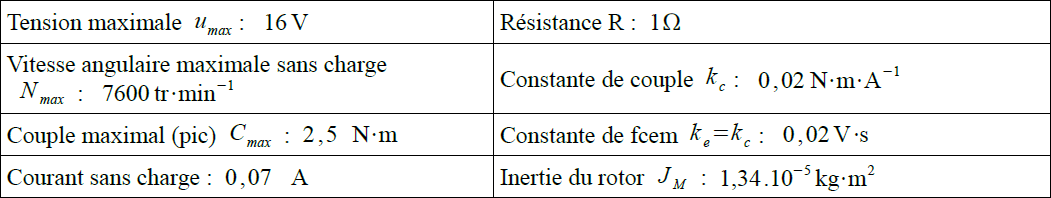
\includegraphics[width=\linewidth]{images/ccmp_06}
%\end{marginfigure}
\fi

\question{À partir des équations caractérisant le système, déterminer les expressions littérales des fonctions
de transfert $H_1( p)$, $H_2 ( p)$, $H_3 ( p)$ et $H_6 ( p)$.}
\ifprof
\begin{corrige}
On a d'une part, $C_M(p)=H_1(p)\left(U_M(p)-\Omega_M(p)\right)$. 

D'autre part, en utilisant les deux équations du moteur électrique, on a $U_M (p)=RI (p)+E(p)$ et $E (p )=k_c \Omega_M (p)$ soit  $U_M (p)=RI (p)+k_c \Omega_M (p)$. De plus $C_M (p)=k_c I (p )$; donc $U_M (p)=R\dfrac{C_M(p)}{k_c}+k_c \Omega_M (p)$. 
Par suite, $C_M(p)=\dfrac{k_c}{R}\left(U_M (p)-k_c \Omega_M (p)\right)$.

En identifiant, on a donc $H_1(p)=\dfrac{k_c}{R}$ et  $H_6(p)={k_c}$.

D'après le schéma-blocs, 

$\Delta \alpha(p) = \left(C(p)-C_M(p)H_2(p)\right)H_3(p)H_4(p)$ soit 

En utilisant l'équation différentielle caractéristique du comportement de la prothèse, on a : 
$J_M p^2 \Delta \alpha(p) + \mu_m p \Delta \alpha(p)  = C_M(p)R_T -C(p)R_T^2$
$\Leftrightarrow \Delta \alpha(p) \left(J_M p^2  + \mu_m p \right)  = C_M(p)R_T -C(p)R_T^2$

$\Leftrightarrow \Delta \alpha(p)  = \dfrac{R_T^2}{J_M p^2  + \mu_m p}\left(\dfrac{C_M(p)}{R_T} -C(p)\right)$.

Or, $\Delta \alpha(p) = \dfrac{1}{p}\Delta \alpha'(p)$; donc $H_4(p)=\dfrac{1}{p}$.

Au final, $H_3(p) = \dfrac{R_T^2}{J_M p  + \mu_m }$ et $H_2(p)=R_T$.

\end{corrige}
\else
\fi

\ifprof
\else

On a par ailleurs $H_4(p)=\dfrac{1}{p}$, $H_5(p)=\dfrac{1}{R_T}$ et $H_7(p)=k_{RS}d_0^2$ ($k_{RS}=\SI{1200e3}{N.m^{-1}}$ raideur équivalente du ressort et $d_0=\SI{0,035}{m}$).

On considère que $\theta(p)=0$. 
\fi

\question{Déterminer la fonction de transfert en boucle fermée $\text{FTBF}(p)=\dfrac{C(p)}{U_M(p)}$.}
\ifprof
\begin{corrige}
On déplace le dernier point de prélèvement avant $H_4$. On ajoute donc $H_4(p)H_7(p)$ dans la retour. 

On a alors $F(p)=\dfrac{\Delta \alpha'(p)}{-} = \dfrac{H_3(p)}{1+H_3(p)H_4(p)H_7(p)}$.
$\text{FTBF}(p)  = \dfrac{H_1(p)H_2(p) F(p)}{1+H_1(p)H_2(p)H_5(p)H_6(p) F(p)}H_4(p)H_7(p) $.

Soit 
$\text{FTBF}(p)  = \dfrac{H_1(p)H_2(p) \dfrac{H_3(p)}{1+H_3(p)H_4(p)H_7(p)}}{1+H_1(p)H_2(p)H_5(p)H_6(p) \dfrac{H_3(p)}{1+H_3(p)H_4(p)H_7(p)}}H_4(p)H_7(p) $

$= \dfrac{H_1(p)H_2(p) H_3(p)}{1+H_3(p)H_4(p)H_7(p)+H_1(p)H_2(p)H_5(p)H_6(p) H_3(p)}H_4(p)H_7(p) $

$= \dfrac{\dfrac{k_c}{R}R_T \dfrac{R_T^2}{J_M p  + \mu_m }}{1+\dfrac{R_T^2}{J_M p  + \mu_m }\dfrac{k_{RS}d_0^2}{p}+\dfrac{k_c}{R}R_T \dfrac{1}{R_T}k_c \dfrac{R_T^2}{J_M p  + \mu_m }}\dfrac{k_{RS}d_0^2}{p} $

$= \dfrac{\dfrac{k_c}{1} R_T^3}{J_MR p^2  + \mu_m R p+R_TR^2k_{RS}d_0^2+pk_ck_c R_T^2}k_{RS}d_0^2 $

$= \dfrac{k_c R_T^3}{J_MR p^2  + p\left(\mu_m R  +k_ck_c R_T^2\right)+R_TR^2k_{RS}d_0^2}k_{RS}d_0^2 $.
\end{corrige}
\else
\fi


%
%\subsection*{Identification d'un modèle de comportement de la chaîne d'énergie}
%
%\begin{obj}
%Le modèle de la chaîne d'énergie étant défini, on cherche maintenant à déterminer plus précisément les
%valeurs numériques des coefficients intervenant dans les fonctions de transfert de la chaîne d'énergie.\end{obj}
%
%\begin{minipage}[c]{.55\linewidth}
%On procède pour cela à une identification fréquentielle du
%comportement de la prothèse. L'expérience consiste à bloquer le
%tibia ainsi que le pied et à envoyer une commande en tension
%sinusoïdale au moteur en faisant varier la fréquence du signal.
%Dans ces conditions, le basculeur se déplace et écrase le ressort.
%On peut alors relever le couple $C$ au niveau de la cheville. On obtient alors les diagrammes de Bode
%donnés dans le document-réponse. Attention,
%l'abscisse est en hertz et le gain est normalisé
%$G_{\text{dB}}=20 \log\left( \dfrac{|H(p)|}{K_0}\right)$ . La courbe en tirets représente le modèle
%du second ordre déterminé précédemment s'approchant au mieux
%des courbes expérimentales.
%\end{minipage} \hfill
%\begin{minipage}[c]{.4\linewidth}
%\begin{marginfigure}
%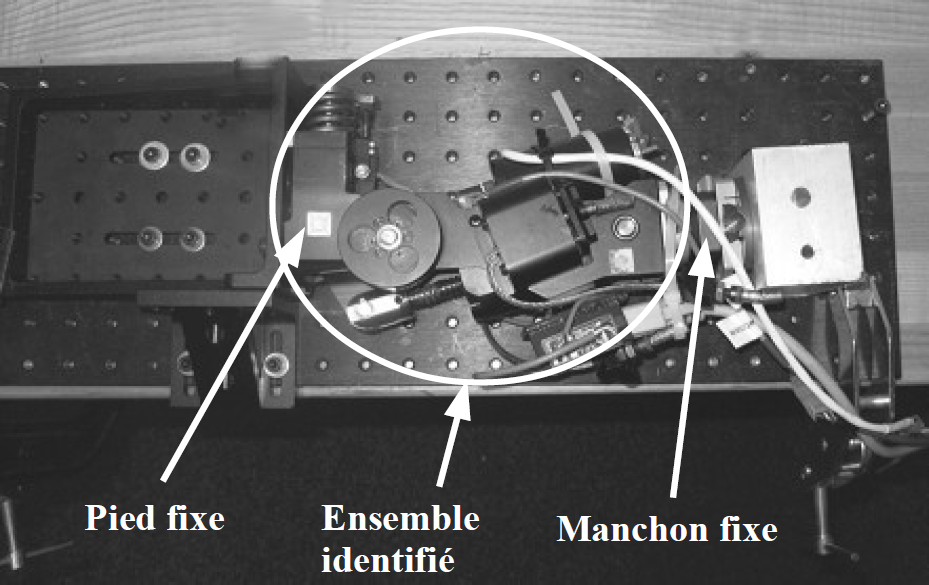
\includegraphics[width=\linewidth]{images/ccmp_03}
%
%\textit{Montage expérimental : pied et tibia (manchon) bloqués}
%\end{marginfigure}
%\end{minipage} 
%
%
%\subparagraph{}
%\textit{Déterminer les valeurs numériques de la pulsation propre non amortie $\omega_0$ et du coefficient
%d'amortissement $\xi_0$ à partir de la représentation approchée (courbe en tirets), en détaillant succinctement
%la méthode utilisée. Les tracés seront faits sur le document-réponse.}
%\ifprof
%\begin{corrige}
%\end{corrige}
%\else
%\fi
%
%\ifprof
%\else
%\newpage
%\if

%
%\subsection*{Contrôler le processus lors de la phase d'appui}
%
%\begin{obj}
%La gestion des modes de commande permet de définir les séquences où l'asservissement s'effectue en
%position et celles où l'asservissement s'effectue en couple. L'objectif de cette partie est de définir l'asservissement
%en couple et d'analyser les performances de cet asservissement.
%\end{obj}
%
%\subsubsection*{Mise en place de l'asservissement en couple}
%\ifprof
%\else
%On se place pour analyser les performances de l'asservissement en couple dans le cadre de l'expérience
%d'identification décrite précédemment (pied et tibia bloqués).
%
%L'asservissement en couple est réalisé grâce à un potentiomètre linéaire qui délivre une tension $u_{\text{mes}}$ image de la
%variation de longueur des ressorts $\Delta X $. On note $K_{\text{capt}}$ le gain de ce capteur. D'autre part, un bloc d'adaptation de gain $K_A$ permet d'obtenir une tension $u_{\text{th}}$ image du couple de consigne $C_{\text{th}}$. L'écart $\varepsilon$ entre les tensions $u_{\text{th}}$ et
%$u_{\text{mes}}$ est corrigé par un correcteur de fonction de transfert $H_c ( p)$ qui délivre la tension $u_M$ au moteur par
%l'intermédiaire de l'amplificateur de gain $K_{\text{amp}}$.
%\fi
%
%
%\question{Compléter le schéma-blocs afin de mettre en place
%l'asservissement en couple. Proposer une expression de $K_A$ permettant de réaliser un asservissement
%correct.}
%\ifprof
%\begin{corrige}
%\end{corrige}
%\else
%\fi
%
%\begin{marginfigure}
%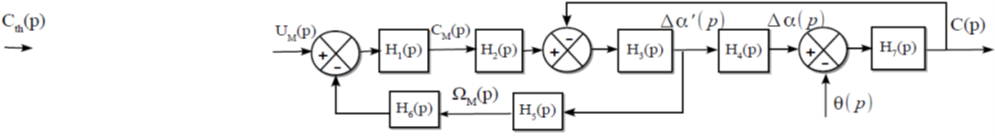
\includegraphics[width=\linewidth]{ccmp_09}
%
%%\textit{Schéma-blocs de l'asservissement en couple simplifié}
%\end{marginfigure}

\subsection*{Analyse des performances de l'asservissement en couple}
\ifprof
\else

%\begin{minipage}[c]{.5\linewidth}
Le schéma-blocs de l'asservissement en couple peut être simplifié par le schéma-blocs suivant avec 
$H( p)=\dfrac{a_0}{1+a_1 p+a_2 p^2}$ où 
$a_0=\SI{2,9}{NmV^{-1}}$, 
$a_1=\dfrac{26}{4356}\SI{}{s}$ et $a_2=\dfrac{1}{4356}\SI{}{s^2}$ et $H_{\text{cor}}( p)=H_c (p)K_{\text{amp}}K_A$.
%\end{minipage} \hfill
%\begin{minipage}[c]{.4\linewidth}
\begin{marginfigure}
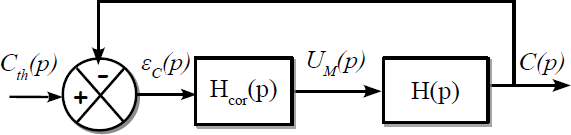
\includegraphics[width=\linewidth]{ccmp_04}

%\textit{Schéma-blocs de l'asservissement en couple simplifié}
\end{marginfigure}
%\end{minipage} 



\begin{obj}
L'objectif est de déterminer si la correction  $H_{\text{cor}}( p)$ permet de respecter le cahier des charges
rappelé ci-après.
\end{obj}

\begin{center}
\begin{tabular}{p{8cm}l}
\hline
Critères & Valeur \\ \hline
Rapidité (temps de réponse à 5\%) & $t_{r5\%}<\SI{0,1}{s}$ \\ 
%Stabilité (marge de phase) & $M_{\varphi}=45\degres$  \\ \hline
Précision pour une entrée en échelon
(écart normalisé par la valeur de l'échelon) & 10 \% maxi \\
\hline
\end{tabular}
\end{center}

%
%
%On choisit dans un premier temps une correction proportionnelle telle que  $H_{\text{cor}}( p)= K_{\text{cor}}$.
%
%
%\subparagraph{}
%\textit{Déterminer l'expression de l'écart statique pour une entrée en échelon unitaire. En déduire la
%valeur de $K_{\text{cor}}$ notée $K_{\text{cor1}}$ qui permette d'assurer le critère du cahier des charges.}
%
%\vspace{.25cm}
%Les diagrammes de Bode de la fonction $H ( p)$ sont donnés dans le document-réponse.
%
%
%
%\subparagraph{}
%\textit{Déterminer graphiquement la valeur du correcteur proportionnel, notée $K_{\text{cor2}}$ pour assurer une
%marge de phase $M_{\varphi}=45\degres$ . Conclure sur l'aptitude du correcteur à vérifier les critères de précision et
%stabilité.}
%
%
%On retient finalement une correction telle que : $H_{\text{cor}}( p)= K_p+K_d \dfrac{\tau_d}{1+\tau_d p}$
%avec $K_p=\SI{4,3}{V.N^{-1}.m^{-1}}$, $K_d=\SI{20,6}{V.N^{-1}.m^{-1}}$ et $\tau_d=\SI{0,0016}{s}$.
%Les diagrammes de Bode de la Fonction de Transfert en Boucle Ouverte (FTBO) corrigée sont donnés sur le
%document-réponse. On réalise également une simulation pour une entrée en échelon de couple de
%\SI{50}{Nm} . La réponse indicielle du couple $C$ ainsi que l'évolution de la tension de commande de la prothèse $u_M$
%au cours du temps sont alors représentées.
%
%\subparagraph{}
%\textit{Tracer le diagramme asymptotique en le justifiant rigoureusement. }

\fi

\question{À l'aide des courbes, valider l'ensemble des critères du cahier des charges en justifiant clairement vos réponses. }

\ifprof
\else
\begin{marginfigure}
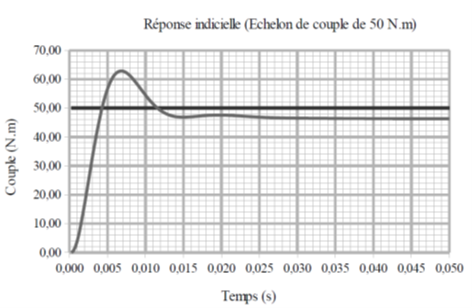
\includegraphics[width=\linewidth]{ccmp_10}
%\textit{Schéma-blocs de l'asservissement en couple simplifié}
\end{marginfigure}
\fi

\ifprof
\begin{corrige}
\begin{itemize}
\item Le régime permanent semble atteint autour de \SI{0,03}{s}; donc les critère de rapidité est respécté.
\item En régime permanent, le couple atteint est de \SI{46}{Nm} pour une consigne de \SI{50}{Nm}. Un écart de 10 \% correspondrait à un couple atteint de \SI{45}{Nm}. Le critère de précision est respecté.
\end{itemize}
\end{corrige}
\else
\fi




\ifprof
\else

\ifcolle
\else
\marginnote{
\begin{solution}
\begin{enumerate}
\item  $H_1(p)=\dfrac{k_c}{R}$, $H_2(p)=R_T$,  $H_3(p) = \dfrac{R_T^2}{J_M p  + \mu_m }$ et   $H_6(p)={k_c}$.
\item $\text{FTBF}(p)= \dfrac{k_c R_T^3}{J_MR p^2  + p\left(\mu_m R  +k_ck_c R_T^2\right)+R_TR^2k_{RS}d_0^2}k_{RS}d_0^2 $.
\item .
\end{enumerate} 
\end{solution}}
\fi

\marginnote{Corrigé voir \ref{B2:07:77}.}

\fi 
 
\graphicspath{{\repStyle/png/}{../SLCI/SLCI-03-SchemaBlocs/78_RobotDaVinci/images/}} 
\normaltrue \difficilefalse \tdifficilefalse
\correctiontrue
%\UPSTIidClasse{11} % 11 sup, 12 spé
%\newcommand{\UPSTIidClasse}{11}

\exer{Conception de la commande d’un robot chirurgical$\star$ \label{B2:07:78}}

% Concours Mines Ponts MP -- PSI --  2013

\setcounter{question}{0}\UPSTIcompetence[2]{B2-07}
\index{Compétence B2-07}
\index{Schéma-blocs}
\index{Robot}
\ifcorrection
\else
\marginnote{\textbf{Pas de corrigé pour cet exercice.}}
\fi




\ifprof
\else
\subsection*{Présentation du système}

Afin d’améliorer les conditions d’opérations chirurgicales dites mini invasives (comme la précision d’opération
et le confort du chirurgien), des robots chirurgicaux ont vu le jour. Cette étude s’intéresse à l’un d’entre eux : le
robot Da Vinci. Le chirurgien peut atteindre sa cible grâce à des outils longs et fins traversant le patient grâce
à une incision de l’ordre du centimètre.


Le système étudié est composé de deux sous-systèmes principaux :
\begin{itemize}
\item l’ensemble \{console de commande + bras maîtres\} permet au chirurgien de visualiser et de commander les
mouvements des outils adéquats à l’intérieur du patient via une caméra haute définition dont l’image est
retransmise par l’intermédiaire d’écrans. Le chirurgien commande les mouvements des outils grâce à deux
bras maîtres dont les extrémités sont maintenues dans chaque main ;
\item les bras esclaves reçoivent les consignes issues du chirurgien par l’intermédiaire des bras maîtres. Il y a au
total 3 bras esclaves : deux manipulent chacun un outil, le troisième manipule une caméra.
\end{itemize}
\begin{center}
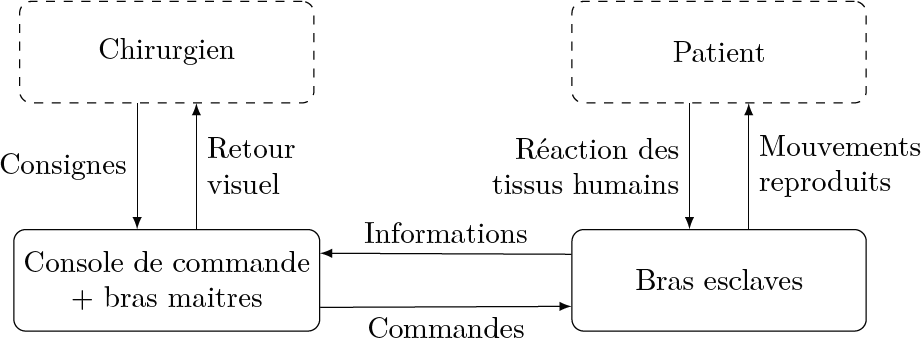
\includegraphics[width=\linewidth]{fig_02}
%\textit{}
\end{center}


Le mouvement de l'axe 1 est régi par l'équation suivante : 
$\Delta C_1(t)=J\dfrac{\dd^2 \Delta \theta_1(t)}{\dd t^2} - k_1 \dfrac{r_9'}{r_0}h_2 \Delta F_x(t)$ avec $J=\SI{1,98e-5}{kg.m^2}$, $k_1\dfrac{r_9'}{r_0}=0,00717$, $h_2=\SI{0,2}{m}$.

Le couple moteur $\Delta C_1(t)$ est fourni par une machine à courant continu modélisée par les équations suivantes : 
$u_1(t)=L\dfrac{\dd i_1(t)}{\dd t}  + Ri_1(t)+e_1(t)$, $e_1(t)=k_e \dfrac{\dd \Delta \theta_1(t)}{\dd t}$, $\Delta C_1(t) = k_t i_1(t)$ avec $u_1(t)$ la tension aux bornes du moteur, $i_1(t)$ l’intensité traversant le moteur et $e_1(t)$ la force contre
électromotrice, avec $R=\SI{2,08}{\Omega}$, $k_t = \SI{0,0525}{N.m.A^{-1}}$ et $k_e = \SI{0,0525}{V.s.rad^{-1}}$.

On fait l’hypothèse que l’influence de l’inductance $L$ est négligeable sur les performances attendues, soit $L=0$.

La consigne est notée $\Delta \theta _{c1}(t)$. Le cahier des charges sélectif conduit à choisir un correcteur associant une anticipation (via la présence de $\sigma_4$ dans la relation suivante) et une correction PID. La tension de commande du moteur est donnée par : $U_1(p)=\left( \Delta \theta_{c1}(p)-\Delta \theta_1(p)\right) \left(\sigma_1 + \dfrac{\sigma_2}{p}\right)- \sigma_3p \Delta \theta_1(p)+\sigma_4\Delta \theta_{c1}(p)$
avec $\Delta \theta_{c1}(p)$ la consigne de position angulaire exprimée dans le domaine symbolique.
\fi


\question{Compléter le schéma-blocs.}
\ifprof
\begin{corrige} ~\\

\begin{center}
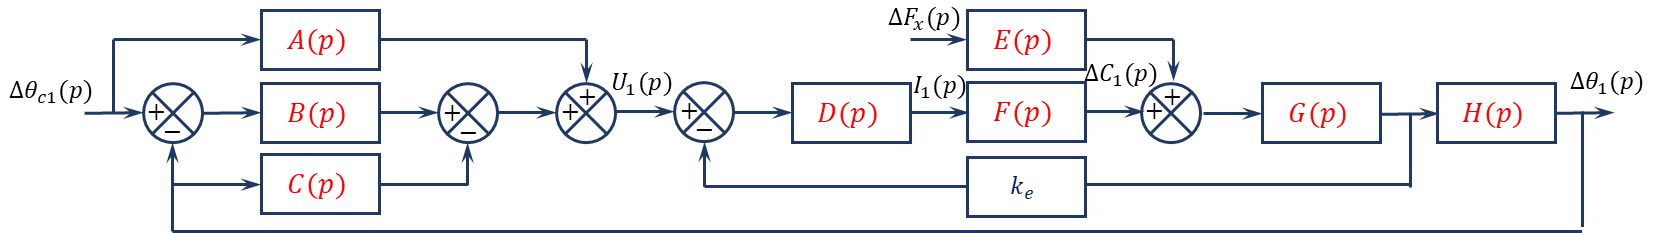
\includegraphics[width=\linewidth]{cor_02}
%\textit{}
\end{center}


En utilisant l'équation électrique du MCC, on a 
$U_1(p)=\left(L p   + R\right)I_1(p)+E_1(p)$. En utilisant le schéma-blocs :  $I_1(p)=\left(U_1(p) - E(p)\right) D(p)$. On a donc 
$I_1(p)=\dfrac{U_1(p) - E(p)}{R+Lp}$ et $D(p) = \dfrac{1}{R+Lp}$.

En utilisant la première relation de comportement du MCC, on a $E_1(p)$ en sortie du bloc $k_e$ et $p\Delta_1(p)$ en entrée; donc $H(p)=\dfrac{1}{p}$.

En utilisant la seconde relation, on a $F(p)=k_t$.

En utilisant l'équation de mouvement de l'axe 1, on a :
$\Delta C_1(p)=J p ^2  \Delta \theta_1(p) - k_1 \dfrac{r_9'}{r_0}h_2 \Delta F_x(p)$.

D'après le schéma-blocs, on a $\Delta \theta_1(p) = \left(\Delta C_1(p)+\Delta F_x(p) E(p)\right) G(p)H(p)$.

En réageançant l'équation, on a 
$J p ^2  \Delta \theta_1(p) = \Delta C_1(p) +  k_1 \dfrac{r_9'}{r_0}h_2 \Delta F_x(p) $
$ \Leftrightarrow   \Delta \theta_1(p) = \left(\Delta C_1(p) +  k_1 \dfrac{r_9'}{r_0}h_2 \Delta F_x(p)\right) \dfrac{1}{J p ^2} $.

On a donc $E(p)= k_1 \dfrac{r_9'}{r_0}h_2 $. 

De plus $G(p)H(p)=\dfrac{1}{Jp^2}$ et $H(p)=\dfrac{1}{p}$; donc $G(p)=\dfrac{1}{Jp}$.


En utilisant l'équation électrique du MCC, on a 
$U_1(p)=\left(L p   + R\right)I_1(p)+E_1(p)$. En utilisant le schéma-blocs :  $I_1(p)=\left(U_1(p) - E(p)\right) D(p)$. On a donc 
$I_1(p)=\dfrac{U_1(p) - E(p)}{R+Lp}$ et $D(p) = \dfrac{1}{R+Lp}$.


En utilisant l'équation du PID, on a 
$U_1(p)=\left( \Delta \theta_{c1}(p)-\Delta \theta_1(p)\right) \left(\sigma_1 + \dfrac{\sigma_2}{p}\right)- \sigma_3p \Delta \theta_1(p)+\sigma_4\Delta \theta_{c1}(p)$
soit $U_1(p)=\left( \Delta \theta_{c1}(p) \left(\sigma_1 + \dfrac{\sigma_2}{p}\right) -\Delta \theta_1(p) \left(\sigma_1 + \dfrac{\sigma_2}{p}\right)\right) - \sigma_3p \Delta \theta_1(p)+\sigma_4\Delta \theta_{c1}(p)$.

En utilisant le schéma-blocs, on a 
$U_1(p)=\Delta_{c1}(p) A(p) + \left(\Delta_{c1}(p) -\Delta\theta_{1}(p)\right) B(p) - \Delta\theta_{1}(p)C(p)$
$=\Delta_{c1}(p) \left( A(p) + B(p)\right) -\Delta\theta_{1}(p)  \left(B(p)+C(p)\right)$.

Par suite, 
$U_1(p)= \Delta \theta_{c1}(p) \left(\sigma_1 + \dfrac{\sigma_2}{p} +\sigma_4\right) -\Delta \theta_1(p) \left(\sigma_1 + \dfrac{\sigma_2}{p} + \sigma_3p\right)$.

On aura donc $B(p)=\sigma_1 + \dfrac{\sigma_2}{p}$, $C(p)=\sigma_3 p$ et  $A(p)=\sigma_4$.


\begin{center}
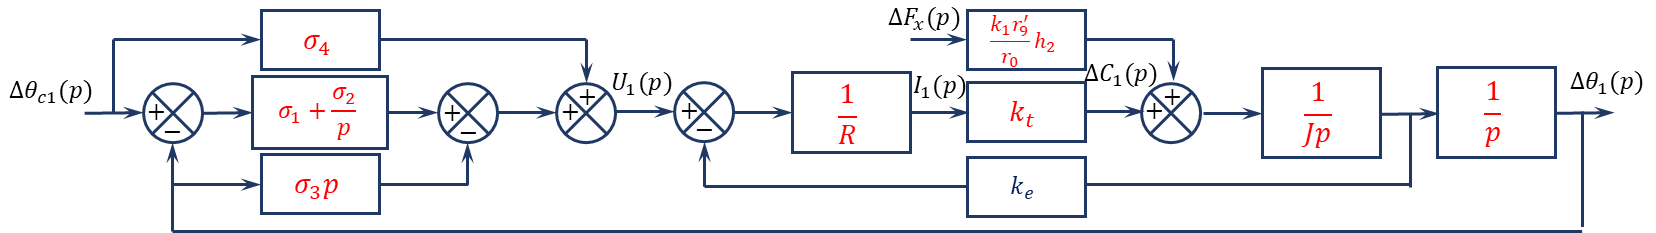
\includegraphics[width=\linewidth]{cor_03}
%\textit{}
\end{center}
\end{corrige}
\else
\fi


\ifprof
\else
Pour la suite, on considère la perturbation nulle ($\Delta F_x(p)=0$).
\fi

\question{À partir de ce schéma-blocs, en notant $H_{\text{processus}}(p)=\dfrac{\Delta \theta_1(p)}{U_1(p)}=\dfrac{K}{p\left(1+\tau p \right)}$, exprimer $K$ et $\tau$ en fonction des données de l'énoncé.}
\ifprof
\begin{corrige}
On a $H_{\text{processus}}(p)= \dfrac{D(p)F(p)G(p)}{1+D(p)F(p)G(p) k_e} H(p)$
soit $H_{\text{processus}}(p)= \dfrac{\dfrac{1}{R+Lp}k_t\dfrac{1}{Jp}}{1+\dfrac{1}{R+Lp}k_t\dfrac{1}{Jp} k_e} \dfrac{1}{p}$.
Avec $L=0$, 
$H_{\text{processus}}(p) =\dfrac{k_t}{RJp+k_t k_e} \dfrac{1}{p}=\dfrac{\dfrac{1}{k_e}}{\dfrac{RJ}{k_t k_e}p+1} \dfrac{1}{p}$ soit $K = \dfrac{1}{k_e}$ et $\tau = \dfrac{RJ}{k_t k_e}$.
\end{corrige}
\else
\fi



\question{Exprimer la fonction de transfert en boucle fermée, sous sa forme canonique, notée $B_F(p) = \dfrac{\Delta \theta_1(p)}{\Delta \theta_{c1}(p)}$ en fonction de $K$, $\tau$, $\sigma_1$, $\sigma_2$, $\sigma_3$ et  $\sigma_4$.}
\ifprof
\begin{corrige}
On a vu que $U_1(p)= \Delta \theta_{c1}(p) \left(\sigma_1 + \dfrac{\sigma_2}{p} +\sigma_4\right) -\Delta \theta_1(p) \left(\sigma_1 + \dfrac{\sigma_2}{p} + \sigma_3p\right)$ et 
que $\dfrac{\Delta \theta_1(p)}{U_1(p)}=\dfrac{K}{p\left(1+\tau p \right)}$.

On a donc 
$\Delta \theta_1(p) \dfrac{p\left(1+\tau p \right)}{K}= \Delta \theta_{c1}(p) \left(\sigma_1 + \dfrac{\sigma_2}{p} +\sigma_4\right) -\Delta \theta_1(p) \left(\sigma_1 + \dfrac{\sigma_2}{p} + \sigma_3p\right)$

$\Leftrightarrow \Delta \theta_1(p) \left(\dfrac{p\left(1+\tau p \right)}{K}  + \sigma_1 + \dfrac{\sigma_2}{p} + \sigma_3p\right)= \Delta \theta_{c1}(p) \left(\sigma_1 + \dfrac{\sigma_2}{p} +\sigma_4\right) $ et 

$B_F(p) = \dfrac{\sigma_1 + \dfrac{\sigma_2}{p} +\sigma_4}{\dfrac{p\left(1+\tau p \right)}{K}  + \sigma_1 + \dfrac{\sigma_2}{p} + \sigma_3p}$ 
$= \dfrac{\sigma_1 p + \sigma_2 + \sigma_4 p}{\dfrac{p^2\left(1+\tau p \right)}{K}  + \sigma_1p + \sigma_2 + \sigma_3p^2}$
$= K \dfrac{\sigma_1 p + \sigma_2 + \sigma_4 p}{p^2\left(1+\tau p \right)  + \sigma_1 K p + \sigma_2 K  + \sigma_3 Kp^2}$
$= K \dfrac{\left(\sigma_1+ \sigma_4 \right) p + \sigma_2 }{ \tau p^3 + p^2\left(1+\sigma_3 \right)  + \sigma_1 K p + \sigma_2 K  }$.
\end{corrige}
\else
\fi



\ifprof
\else
\begin{center}
\rotatebox{90}{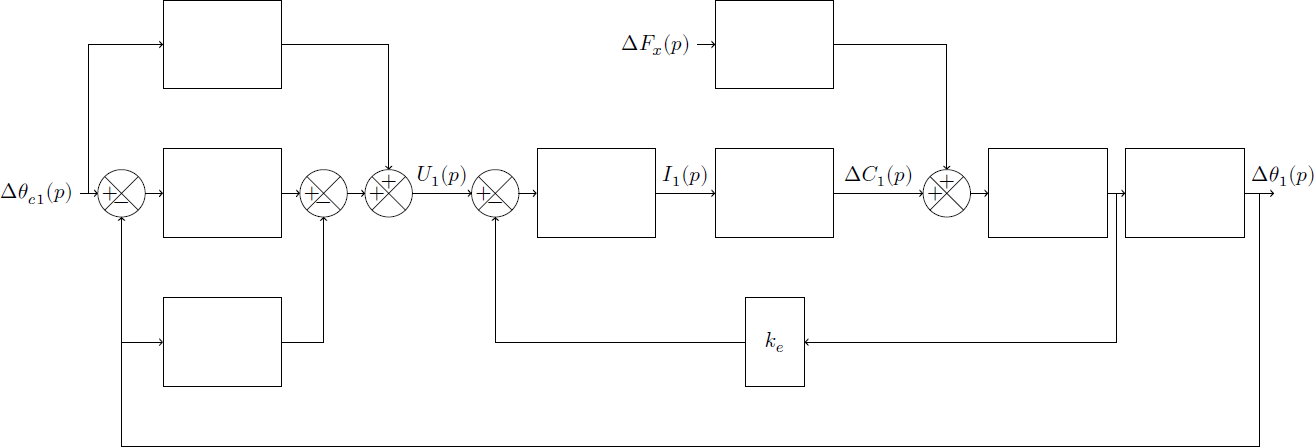
\includegraphics[height=.9\linewidth]{fig_03}}
%\textit{Schéma-blocs de l'asservissement du dosseret \label{fig6}}
\end{center}
\fi


\ifprof
\else
\footnotesize
\begin{tabular}{|p{.95\linewidth}|}
\hline
\begin{enumerate}
\item 
$A(p)=\sigma_4$,
$B(p)=\sigma_1 + \dfrac{\sigma_2}{p}$, 
$C(p)=\sigma_3 p$, 
$D(p) = \dfrac{1}{R+Lp}$, 
$E(p)= k_1 \dfrac{r_9'}{r_0}h_2 $, 
$F(p)=k_t$, 
$G(p)=\dfrac{1}{Jp}$, 
$H(p)=\dfrac{1}{p}$.
\item $K = \dfrac{1}{k_e}$ et $\tau = \dfrac{RJ}{k_t k_e}$.
\item $B_F(p) = K \dfrac{\left(\sigma_1+ \sigma_4 \right) p + \sigma_2 }{ \tau p^3 + p^2\left(1+\sigma_3 \right)  + \sigma_1 K p + \sigma_2 K  }$.
\end{enumerate} \\
\hline
\end{tabular}
\normalsize
\begin{flushright}
\footnotesize{Corrigé  voir \ref{B2:07:78}.}
\end{flushright}%
\fi 
 
\graphicspath{{\repStyle/png/}{../SLCI/SLCI-03-SchemaBlocs/79_Tuyere/images/}} 
\normaltrue \difficilefalse \tdifficilefalse
\correctionfalse

%\UPSTIidClasse{11} % 11 sup, 12 spé
%\newcommand{\UPSTIidClasse}{11}

\exer{Tuyère à ouverture variable$\star$ \label{B2:07:79}}

% Concours Banque PT SIA -  2011

\setcounter{question}{0}\marginnote{\xpComp{SLCI}{03}}%\UPSTIcompetence{B2-07}
\index{Compétence B2-07}\index{Compétence SLCI-03}
\index{Schéma-blocs}
\index{Robot}
\ifcorrection
\else
\marginnote{\textbf{Pas de corrigé pour cet exercice.}}
\fi


\subsection*{Présentation du système}
\ifprof
\else
Les propulseurs utilisés dans les applications militaires ou civiles subissent, des tests de certification
visant à contrôler leur bon fonctionnement et le respect des normes de sécurité.

Ces tests consistent à simuler au sol les conditions de vol subies par le propulseur et à observer les réactions de celui-ci
consécutives à des commandes de pilotage. 

La DGA (Direction Générale de l'Armement) dispose dans son centre d'essais des propulseurs de bancs d'essais
dédiés à la certification et à la mise au point de différents types de propulseurs d'avions ou de missiles.

\begin{marginfigure}
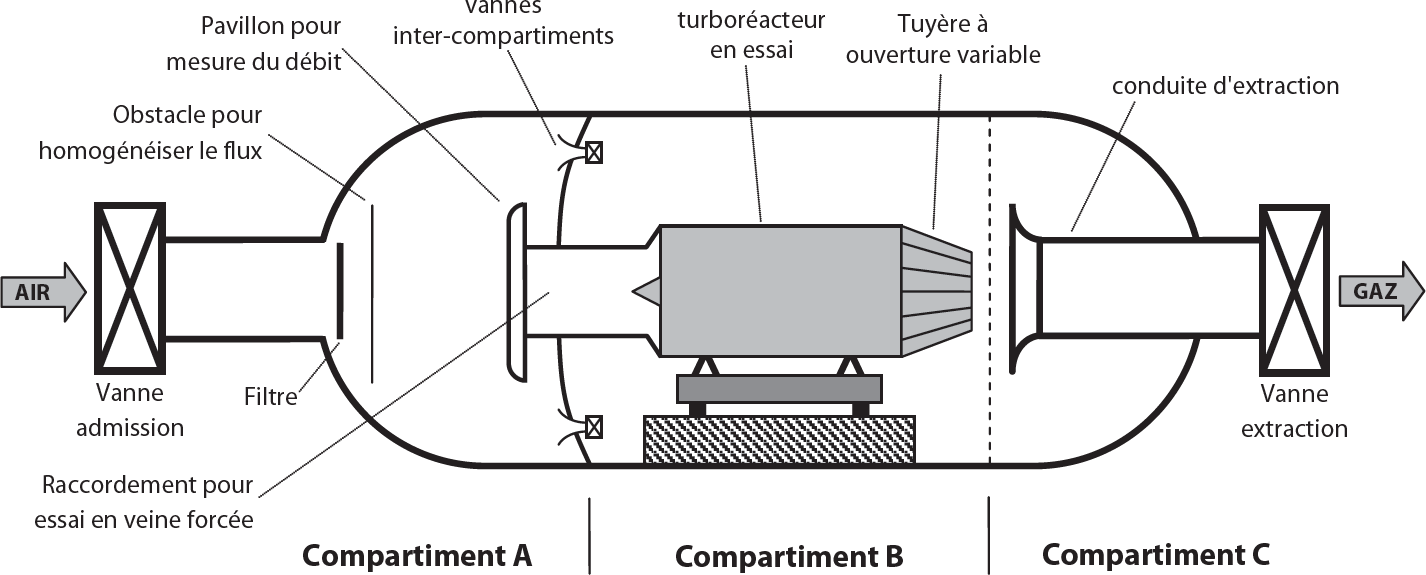
\includegraphics[width=\linewidth]{fig_02}
%\textit{}
\end{marginfigure}

Le banc d'essai est composé d'un tube représentant le corps du réacteur et d'une tuyère à ouverture variable
actionnée par quatre vérins hydrauliques et permettant de faire varier la vitesse de l'air éjecté. 

%\begin{marginfigure}
%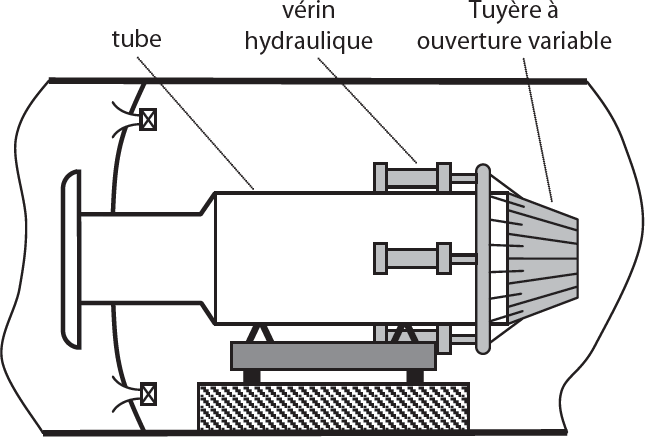
\includegraphics[width=.8\linewidth]{fig_03}
%%\textit{}
%\end{marginfigure}

\begin{marginfigure}
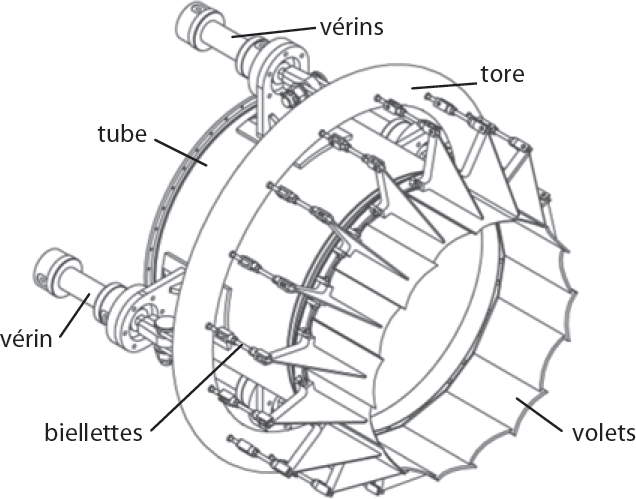
\includegraphics[width=.8\linewidth]{fig_04}
%\textit{}
\end{marginfigure}

\fi

\begin{obj}
On souhaite vérifier que le système permet de respecter le cahier des charges suivant : 
\begin{itemize}
\item temps de réponse à 5\% : \SI{4}{s} au maximum;
\item précision : l'erreur statique doit être nulle;
\item précision : l'erreur de traînage doit être inférieure à \SI{1}{mm} pour une consigne de \SI{25}{mm.s^{-1}}.
\end{itemize}
\end{obj}


\subsection*{Modélisation du comportement du vérin -- hypothèse fluide compressible}
\ifprof
\else

\begin{obj}
Il s'agit ici de proposer un modèle plus affiné du comportement du vérin en tenant compte de la compressibilité du fluide et du comportement dynamique du mécanisme.
\end{obj}		



Pour rendre compte du comportement dynamique du système on propose un modèle de comportement du vérin en tenant compte de la compressibilité du fluide. L'évolution du débit est alors une fonction du déplacement mais aussi de la pression sous la forme de la relation suivante : $q(t)=S\dfrac{\dd x(t)}{\dd t}+\dfrac{V_0}{B}\dfrac{\dd \sigma(t)}{\dd t}$ avec : 
\begin{itemize}
\item $\sigma(t)$ : pression utile dans le vérin. On notera $\Sigma(p)$ sa transformée;
\item $V_0$ : demi volume de fluide contenu dans le vérin;
\item $B$ : coefficient de compressibilité du fluide.
\end{itemize}  

La pression utile induit l'effort développé par le vérin que nous noterons $F_v$ tel que : $F_V(p)=S\Sigma(p)$ où $S$ représente la section utile du vérin en sortie de tige.

$V(p)$ représente l'image par la transformation de Laplace de la vitesse de translation $v(t)$ de la tige du vérin. 

En considérant les actions de pesanteur négligeables et en se plaçant dans une phase de test à vide (sans flux d'air), l'application des lois de la dynamique donne la relation suivante : $F_V(t)=M_{\text{eq}} \dfrac{\dd^2 x(t)}{\dd t^2}$.

\fi 

\question{À partir des équations, compléter le schéma-blocs en indiquant les fonctions de transferts de chaque bloc.}
\ifprof
\begin{corrige} ~\\
\begin{center}
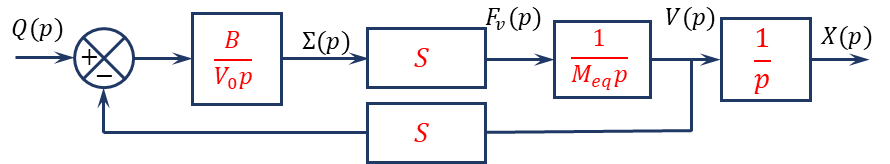
\includegraphics[width=.95\linewidth]{cor_01_b}
%\textit{}
\end{center}

\end{corrige}
\else
\
\begin{marginfigure}
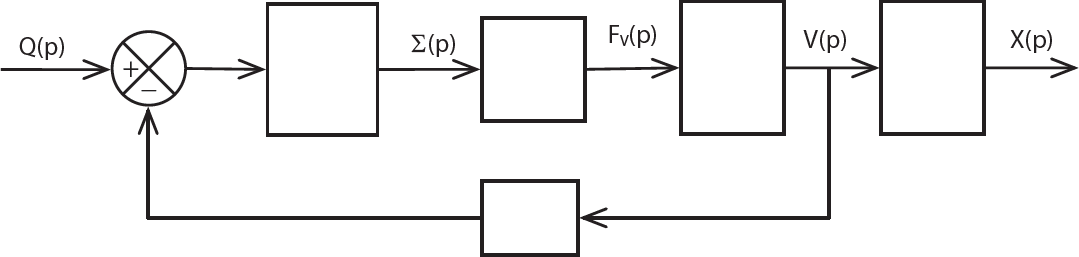
\includegraphics[width=\linewidth]{fig_05}
%\textit{}
\end{marginfigure}

On note $F_R$ l'action mécanique résistante équivalente pour quatre volets. On a $F_R(t) = K_F x(t)$. L'application du théorème de l'énergie cinétique se traduit par $M_{\text{eq}}\ddot{x}(t)=\left(F_V(t)-F_R(t)\right)$. 
\fi

\question{Modifier le schéma-blocs précédent pour intégrer l'effort résistant.}
\ifprof
\begin{corrige} ~\\
\begin{center}
\includegraphics[width=.95\linewidth]{cor_02_b}
\end{center}
\end{corrige}
\else
\fi

\question{Donner l'expression de la fonction de transfert du vérin $H_V(p)=\dfrac{X(p)}{Q(p)}$. On donnera le résultat sous la forme $H_V(p)=\dfrac{K_V}{p\left(1+a_2 p^2 \right)}$ en précisant les expression de $K_V$ et $a_2$.}
\ifprof
\begin{corrige} ~\\
\begin{center}
\includegraphics[width=\linewidth]{cor_03}
\end{center}
\end{corrige}
\else
\fi

\subsection*{Validation du comportement du vérin} 

\ifprof
\else

Afin de valider le modèle établi, on se propose d'étudier le comportement en boucle fermée de la chaîne fonctionnelle de commande du vérin. On rappelle ci-dessous le schéma-bloc retenu et on considérera une correction proportionnelle telle que  $C(p)=K_p$.

\begin{center}
\includegraphics[width=\linewidth]{fig_06}
%\textit{}
\end{center}
\fi

\question{Donner  l'expression de la forme canonique de la fonction de transfert en boucle fermée $H_{\text{BF}}(p)=\dfrac{X(p)}{X_{\text{ref}}(p)}$ . On donnera le résultat en fonction de $K_C$, $K_U$, $K_D$, $K_p$, $K_V$ et $a_2$. }
\ifprof
\begin{corrige} ~\\
\begin{center}
\includegraphics[width=.5\linewidth]{cor_04}
\end{center}
\end{corrige}
\else
\fi

\subsection*{Prise en compte du débit de fuite} 
\ifprof
\else

Pour pallier le problème de stabilité du modèle précédemment établi, une solution possible consiste à un introduire un débit de fuite entre les deux chambres du vérin. Celui-ci a pour effet de réduire artificiellement le débit réel entrant dans le vérin en fonction de la pression utile. Ce débit vaut alors : $q(t)-\delta \sigma (t)$  où $\delta$ est le coefficient de débit de fuite.
\fi

\ifprof
\newpage
\else \fi

\question{Modifier le schéma-blocs précédent pour intégrer le débit de fuite.}
\ifprof
\begin{corrige} ~\\
\begin{center}
\includegraphics[width=.95\linewidth]{cor_03_b}
\end{center}
\end{corrige}
\else
\fi


\question{Donner l'expression de la fonction de transfert du vérin $H_V(p)=\dfrac{X(p)}{Q(p)}$. On donnera le résultat sous la forme $H_V(p)=\dfrac{K_V}{p\left(1+a_1 p + a_2 p^2+ a_3 p^3 \right)}$ en précisant les expression de $K_V$, $a_1$, $a_2$ et $a_3$.}
\ifprof
\begin{corrige} ~\\
\begin{center}
\includegraphics[width=.5\linewidth]{cor_06}
\end{center}
\end{corrige}
\else
\fi
\subsection*{Retour sur le cahier des charges}
On donne la réponse à un échelon et à une rampe de pente \SI{25}{mm.s^{-1}}.

\question{Le cahier des charges est-il vérifié ?}


\begin{marginfigure}
\includegraphics[width=\linewidth]{echelon}
\includegraphics[width=\linewidth]{rampe}
%\textit{}
\end{marginfigure}




\ifprof
\else

\marginnote{Corrigé voir \ref{B2:07:79}.}

\fi 
 
\graphicspath{{\repStyle/png/}{../SLCI/SLCI-03-SchemaBlocs/80_Clever/images/}} 
\normaltrue \difficilefalse \tdifficilefalse
\correctionfalse

%\UPSTIidClasse{11} % 11 sup, 12 spé
%\newcommand{\UPSTIidClasse}{11}

\exer{Véhicule à trois roues Clever$\star$ \label{B2:07:80}}

% Concours Banque PT SIA -  2011

\setcounter{question}{0}\UPSTIcompetence[2]{B2-07}
\index{Compétence B2-07}
\index{Schéma-blocs}
\index{Clever}
\ifcorrection
\else
\marginnote{\textbf{Pas de corrigé pour cet exercice.}}
\fi

\ifprof
\else
\section*{Présentation du système}

Le Clever est un démonstrateur technologique développé par un tissu d'industriels européens. Clever est la contraction de Compact Low Emission VEhiclefor uRban tRansportation (véhicule compacte à faibles émissions pour le transport urbain) car, avec une consommation de seulement \SI{2,5}{L}/\SI{100}{km}, il s'annonce très écologique. 

L'habitacle peut s'incliner grâce à un système constitué 
\begin{itemize}
\item d'un calculateur qui détermine le mouvement et la position à donner à l'habitacle en fonction des conditions d'utilisation ;
\item d'un système hydro-mécanique de transmission de puissance et d'adaptation de mouvement ;
\item d'un système de contrôle de l'inclinaison de l'habitacle.
\end{itemize}

\begin{center}
\includegraphics[width=.47\linewidth]{fig_02}
\includegraphics[width=.47\linewidth]{fig_03}
%\textit{}
\end{center}

%La chaîne de transmission de puissance et d'adaptation de mouvement est composée :
%\begin{itemize}
%\item d'une pompe à engrenages actionnée par le moteur à gaz via un système de poulies/courroie ;
%\item d'un circuit hydraulique ;
%\item de 2 vérins hydrauliques simple effet ;
%\item d'un système mécanique d'adaptation de mouvement afin de transformer le mouvement de translation des tiges des vérins en rotation de l'habitacle.
%\end{itemize}
\begin{obj}
L'objectif est que le mouvement de l'habitacle soit contrôlé :
\begin{itemize}
\item écart statique : 0\degres;
\item écart de traînage pour une entrée en rampe unitaire : 0\degres;
\item temps de réponse à 5\% : inférieur à \SI{0,1}{s}.

\end{itemize}
\end{obj}

\subsection*{Modélisation du servo-distributeur et du vérin}

L'orientation de l'habitacle est contrôlée par un asservissement de la position angulaire. L'architecture de cet asservissement est représentée par le schéma-blocs de le figure suivante.

On modélise le comportement du servo-distributeur par un gain pur noté $K_s$ et le capteur par $H_c(p)=C$ avec $C=\SI{1}{V.rad^{-1}}$.  L'adaptateur mécanique a un comportement linéaire sur l'intervalle d'utilisation. On a donc $H_{\text{am}}(p)=R$ ($R=\SI{7}{rad.m^{-1}}$). Enfin, on considère que $H_r(p)=1$. 

\begin{center}
\includegraphics[width=\linewidth]{fig_05}
\end{center}

À ce stade de l'étude, le modèle de comportement du fluide correspond à un comportement incompressible. L'équation caractérisant le comportement du vérin est alors : $q(t)=S\dot{\lambda}(t)$ où :
\begin{itemize}
\item $S$ représente la section utile du vérin en sortie de tige (diamètre \SI{32}{mm});
\item $q$ est le débit en entrée de vérin ;
\item $v(t)=\dot{\lambda}(t)=\dfrac{\dd \lambda(t) }{\dd t}$ est la vitesse de translation de la tige du vérin par rapport au corps.
\end{itemize}
% 
\fi

\question{Donner l'expression de la fonction de transfert du vérin $H_{V1}(p)$ (telle que $\lambda(p) = H_{V1}(p) Q(p)$) et compléter le schéma-bloc associé à la modélisation actuelle du système.}
\ifprof
\begin{corrige} ~\\

\begin{center}
\includegraphics[width=.95\linewidth]{cor_01}
%\textit{}
\end{center}
\end{corrige}
\else
\fi

\question{Déterminer la fonction de transfert en boucle fermée $\text{FTBF}_1$ (telle que $\alpha(p) = \text{FTBF}_1(p) \alpha_c(p)$) du système bouclé. Mettre  $\text{FTBF}_1(p)$ sous la forme 
$\dfrac{K_1}{1+\tau_1 p}$ en précisant les expressions de $K_1$ et de $\tau_1$.} 
 \ifprof
\begin{corrige} ~\\

\begin{center}
\includegraphics[width=.95\linewidth]{cor_02}
%\textit{}
\end{center}
\end{corrige}
\else
\fi


\question{ À partir du critère de temps de réponse à 5\% $(t_{r5\%})$ du système, déterminer l'expression puis la valeur numérique minimale du gain du servo-distributeur.} 

\ifprof
\begin{corrige}~\\
\begin{center}
\includegraphics[width=.95\linewidth]{cor_03}
%\textit{}
\end{center}    
\end{corrige}
\else
\fi

\ifprof
\else
\subsection*{Modélisation du comportement du vérin avec fluide compressible et du comportement dynamique du mécanisme}

La compressibilité du fluide étant prise en compte dans le modèle, l'évolution du débit est une fonction du déplacement mais aussi de la pression sous la forme de la relation (1). L'effort exercé par le vérin en sortie de tige est décrit par la relation (2).
$$
q(t)=S\dot{\lambda}(t)+\dfrac{V_0}{B}\dot{p}_r(t) \quad (1) \quad\quad
F_V(t)=Sp_r(t) \quad (2)
$$
où:
\begin{itemize}
\item $p_r(t)$ : pression utile dans le vérin ;
\item $V_0$ : volume caractéristique moyen de fluide contenu dans le vérin et les durites, $V_0 = \SI{2,5e5}{m^3}$;
\item $B$ : coefficient de compressibilité du fluide, $B = \SI{109}{Pa}$;
\item $F_v(t)$ : effort développé par le vérin en sortie de tige ;
\item $S$ : section utile du vérin en sortie de tige.
\end{itemize}

Par ailleurs, $F_v(t)+k_g \lambda(t)=m_{\text{eq}}\ddot{\lambda}(t)$ avec $m_{\text{eq}}$ la masse équivalente du système, $k_g$ une constante, $\lambda(t)$ le déploiement des vérins.
\fi


\question{Appliquer la transformation de Laplace aux équations précédentes et compléter le schéma-blocs.}
\ifprof
\begin{corrige}
\begin{center}
\includegraphics[width=.95\linewidth]{cor_04}
%\textit{}
\end{center}    
\end{corrige}
\else
\fi
\begin{center}
\includegraphics[width=\linewidth]{fig_06}
%\textit{}
\end{center}


\ifprof
\else
\subsection*{Analyse du comportement global}
\fi


\question{Donner l'expression de la fonction de transfert en boucle fermée du vérin $H_{\text{V2}}$ (telle que $\lambda(p) =  H_{\text{V2}} Q(p)$) et préciser les expressions des coefficients $K_V$ et $\omega_V$ de sa forme canonique : $H_{\text{V2}}(p)=\dfrac{K_V}{p\left( 1+\dfrac{p^2}{\omega_V^2}\right)}$.}
\ifprof
\begin{corrige} ~\\
\begin{center}
\includegraphics[width=.95\linewidth]{cor_05}
\includegraphics[width=.95\linewidth]{cor_06}
%\textit{}
\end{center}
\end{corrige}
\else
\fi


\ifprof
\else

\textbf{$k_g$ peut maintenant être négligé.}

\subsection*{Modélisation du comportement dynamique avec prise en compte d'un débit de fuite}
Pour pallier le problème de stabilité du modèle précédemment établi, une solution possible consiste à introduire un débit de fuite au niveau du vérin. Celui-ci a pour effet de réduire artificiellement le débit réel entrant dans le vérin en fonction de la pression utile. L'expression du débit est alors : 
$q(t)=S\dot{\lambda}(t)+\dfrac{V_0}{B} \dot{p}_r(t)-\delta p_r(t)$ où $\delta$ représente le coefficient de débit de fuite.
\fi


\question{Proposer une modification du schéma-bloc donné afin de prendre en compte le débit de fuite.}
\ifprof
\begin{corrige}
\begin{center}
\includegraphics[width=.95\linewidth]{cor_07}
%\textit{}
\end{center}
\end{corrige}
\else
\fi
\begin{center}
\includegraphics[width=\linewidth]{fig_08}
%\textit{}
\end{center}


\question{Déterminer l'expression de la fonction de transfert $H_{V3}$ (telle que $\lambda(p) =  H_{V3} Q(p)$) associée au comportement dynamique du vérin ainsi modélisé. On donnera le résultat sous la forme suivante : 
$H_{V3}(p)=\dfrac{K_V}{p\left(1+a_1 p + \dfrac{p^2}{\omega_V^2} \right)}$.  
Donner l'expression de $a_1$ en fonction de $M_{eq}$, $\delta$ et $S$ et déterminer l'expression du coefficient d'amortissement $\xi_V$ du second ordre en fonction de $M_{\text{eq}}$, $\delta$, $S$, $B$ et $V_0$.}
\ifprof
\begin{corrige}
\begin{center}
\includegraphics[width=.95\linewidth]{cor_08}
%\textit{}
\end{center}
\end{corrige}
\else
\fi

\ifprof
\else
\subsection*{Retour sur le cahier des charges}
Le régulateur étant a priori optimisé, on réalise un essai de validation du comportement temporel de l'inclinaison de l'habitacle, le véhicule étant à l'arrêt. Le calculateur envoie un signal de consigne représentant l'évolution de la position angulaire souhaitée (de 0 à 45\degres en \SI{0,75}{s}). 

\begin{center}
\includegraphics[width=\linewidth]{fig_09}
%\textit{}
\end{center}
\fi

\question{Quels sont les critères du cahier des charges validés ?}
\ifprof
\begin{corrige}
\begin{center}
\includegraphics[width=.95\linewidth]{cor_10}
%\textit{}
\end{center}

\end{corrige}
\else
\fi



\ifprof
\else
\begin{flushright}
\footnotesize{Corrigé  voir \ref{B2:07:80}.}
\end{flushright}%
\fi 
 
\section{Modéliser un SLCI en utilisant un modèle polyphysique} 
\section{Modéliser un SLCI à plusieurs entrées, sous forme matricielle éventuellement} 
\section{Linéariser un comportement, une équation, simplifier un modèle} 
\section{Modéliser un système d'ordre 1 et d'ordre 2  (modèles de connaissance et de comportement)} 
\graphicspath{{\repStyle/png/}{../SLCI/SLCI-07-Ordre12/502_Divers/images/}} 
\normaltrue \difficilefalse \tdifficilefalse
\correctiontrue

%\UPSTIidClasse{11} % 11 sup, 12 spé
%\newcommand{\UPSTIidClasse}{11}

\newpage
\exer{Identification temporelle $\star$ \label{B2:06:502}}
\setcounter{question}{0}\marginnote{\xpComp{SLCI}{07}}%\UPSTIcompetence[2]{B2-06}
\index{Compétence B2-06}
\index{Identification}
\index{Identification temporelle}
\index{Ordre 1}
\index{Ordre 2}
\ifcorrection
\else
\marginnote{\textbf{Pas de corrigé pour cet exercice.}}
\fi


\ifprof 
\else
Soit la réponse à un échelon sur la figure \ref{dds_fig_502_01}.
\begin{marginfigure}
\includegraphics[width=\linewidth]{502_01}
\caption{Réponse à un échelon \label{dds_fig_502_01}}
\end{marginfigure}
\fi

\question{Déterminer la fonction de transfert du système.}
\ifprof
\begin{marginfigure}
\includegraphics[width=8cm]{502_01_cor}
\end{marginfigure}

La tangente à l'origine est non nulle. Il n'y a pas de dépassement. On va donc identifier un système d'ordre 1 de la forme $H(p)=\dfrac{K}{1+\tau p}$.

L'échelon d'entrée a une amplitude de 2. En régime permanent la valeur atteinte est de 7. On a donc $K = \dfrac{7}{2}=3,5$.

Pour identifier la constante de temps, on peut : 
\begin{itemize}
\item regarder à quel temps a lieu l'intersection entre l'asympote en régime permanent et la tangente à l'origine;

\item mesurer le temps de temps réponse à 63\,\%;

\item mesurer le temps de temps réponse à 95\,\% et diviser cette valeur par 3.
\end{itemize}

On a donc $H(p)=\dfrac{3,5}{1+8p}$.
\else
\fi



\ifprof 
\else
Soit la réponse à un échelon d'amplitude 2,5 (figure \ref{dds_fig_502_02}).

\begin{marginfigure}
\includegraphics[width=\linewidth]{502_02}
\caption{Réponse à un échelon d'amplitude 2,5 \label{dds_fig_502_02}}
\end{marginfigure}
\fi

\question{Déterminer la fonction de transfert du système en réalisant les mesures nécessaires et en utilisant les formules appropriées.}
\ifprof
\begin{marginfigure}
\includegraphics[width=8cm]{502_02_cor}
\end{marginfigure}

La tangente à l'origine est nulle et il y a des dépassements. On modélise le système par un système d'ordre 2. 
$H(p)=\dfrac{K}{1+\dfrac{2\xi}{\omega_0}p+\dfrac{p^2}{\omega_0^2}}$.

On a $K= \dfrac{1,25}{2,5}=0,5$.


On mesure un dépassement de 
$1,38 = e^{\dfrac{-\pi \xi}{\sqrt{1-\xi^2}}}$
$\Leftrightarrow \ln 0,38 = \dfrac{-\pi \xi}{\sqrt{1-\xi^2}}$
$\Leftrightarrow \sqrt{1-\xi^2} \ln 1,38 = -\pi \xi$
$\Leftrightarrow (1-\xi^2) (\ln 1,38)^2= \pi^2 \xi^2$
$\Leftrightarrow (\ln 1,38)^2-\xi^2(\ln 1,38)^2 = \pi^2 \xi^2$
$\Leftrightarrow (\ln 1,38)^2 = \pi^2 \xi^2 + \xi^2(\ln 1,38)^2$
$\Leftrightarrow (\ln 1,38)^2 =\xi^2 \left(\pi^2  + (\ln 1,38)^2\right)$
$\Leftrightarrow \dfrac{(\ln 1,38)^2}{\pi^2  + (\ln 1,38)^2} =\xi^2 $
$\Leftrightarrow \xi = \sqrt{\dfrac{(\ln 1,38)^2}{\pi^2  +(\ln 1,38)^2}} =0,3 $.


Par ailleurs, $\omega_0 = \dfrac{2\pi }{T_p \sqrt{1-\xi^2}} =\dfrac{2\pi }{0,44 \sqrt{1-0,3^2}} = \SI{14,9}{rad.s^{-1}}$.

Au final, $H(p)=\dfrac{0,5}{1+\dfrac{2\times 0,3}{14,9}p+\dfrac{p^2}{14,9^2}}$.


\else
\fi



\question{Déterminer la fonction de transfert du système en utilisant les abaques.}
\ifprof
Le dépassement est de 38 \%. On a donc $\xi = 0,3$.

De plus, on mesure $T_{5\%}\times \omega_0 =8$ avec $T_{5\%}=\SI{0,51}{s}$ on a $\omega_0 = 8/0,5 \simeq \SI{16}{rad.s^{-1}}$.

Au final, $H(p)=\dfrac{0,5}{1+\dfrac{2\times 0,3}{16}p+\dfrac{p^2}{16^2}}$.
\begin{center}
\includegraphics[width=\linewidth]{502_03_cor}
\includegraphics[width=\linewidth]{502_04_cor}
\includegraphics[width=\linewidth]{502_05_cor}
\end{center}
\else
\begin{marginfigure}
\includegraphics[width=\linewidth]{502_03}
\end{marginfigure}
\begin{marginfigure}
\includegraphics[width=\linewidth]{502_04}
\end{marginfigure}
\fi


\ifprof
\else
\begin{solution}
\begin{enumerate}
\item  $H(p)=\dfrac{3,5}{1+8p}$.
\item $H(p)=\dfrac{0,5}{1+\dfrac{2\times 0,1}{14,25}p+\dfrac{p^2}{14,25^2}}$.
\item $H(p)=\dfrac{0,5}{1+\dfrac{2\times 0,3}{16}p+\dfrac{p^2}{16^2}}$.
\end{enumerate}
\end{solution}

\marginnote{Corrigé voir \ref{B2:06:502}.}

\fi 
 
\graphicspath{{\repStyle/png/}{../SLCI/SLCI-07-Ordre12/503_Divers/images/}} 
\normaltrue \difficilefalse \tdifficilefalse
\correctiontrue

%\UPSTIidClasse{11} % 11 sup, 12 spé
%\newcommand{\UPSTIidClasse}{11}

\exer{Identification $\star$ \label{B2:06:503}}
\setcounter{question}{0}\marginnote{\xpComp{SLCI}{07}}%\UPSTIcompetence[2]{B2-06}
\index{Compétence B2-06}
\index{Identification}
\index{Identification Bode}
\index{Identification fréquentielle}
\index{Réponse fréquentielle}

\ifcorrection
\else
\marginnote{\textbf{Pas de corrigé pour cet exercice.}}
\fi


\ifprof 
\else

\marginnote{D'après Florestan Mathurin.}

Soit un système dont le diagramme de Bode est donné ci-dessous.
\begin{marginfigure}
\includegraphics[width=\linewidth]{503_01}
\end{marginfigure}
\fi

\question{Tracer le diagramme de Bode asymptotique.}
\ifprof
\begin{marginfigure}
\includegraphics[width=8cm]{503_01_cor}
\end{marginfigure}
\else
\fi


\question{Identifier le type de la fonction de transfert et ses valeurs remarquables.}
\ifprof
La phase tend vers 0 lorsque $\omega$ tend vers \SI{0}{rad/s} et vers $-180\degres$ lorsque $\omega$ tend vers l'infini. 
On observe de plus une résonance. Par ailleurs le gain est nul quand $\omega$ tend vers \SI{0}{rad/s}. 
Le système est donc d'ordre 2 avec un gain unitaire et un $\xi<\dfrac{\sqrt{2}}{2}$. 
On détermine $\omega_0$ lorsque la phase vaut $-90\degres$.

À ce stade, $H(p)=\dfrac{1}{1+\dfrac{2\xi}{4,5}p+\dfrac{p^2}{4,5^2}}$.

Enfin, on mesure un gain à la résonance de \SI{7}{dB}. 
On a donc $20\log A_{\text{max}}=7$ soit $A_{\text{max}}=10^{7/20}= \dfrac{1}{2\xi\sqrt{1-\xi^2}}$.

Par suite, 
 $\dfrac{1}{A_{\text{max}}}=2\xi\sqrt{1-\xi^2}$
 $\Leftrightarrow \dfrac{1}{A_{\text{max}}}=4\xi^2\left(1-\xi^2\right)$
 $\Leftrightarrow \dfrac{1}{A^2_{\text{max}}}=4\xi^2-4\xi^4$
  $\Rightarrow 4\xi^4 -4\xi^2+ \dfrac{1}{A^2_{\text{max}}}=0$ 
  $\Rightarrow 4X^2 -4X+ \dfrac{1}{A^2_{\text{max}}}=0$
  
 On a alors $\Delta = 16 -  \dfrac{16}{A^2_{\text{max}}}$ et $X_{1,2} = \dfrac{4\pm\sqrt{\Delta}}{16}$
 
 En réalisant les applications numériques, on a $\xi = \sqrt{\dfrac{4-\sqrt{\Delta}}{16}} = 0,23$.
  
Alors, $H(p)=\dfrac{1}{1+\dfrac{2\times 0,23}{4,5}p+\dfrac{p^2}{4,5^2}}$.
\begin{marginfigure}
\includegraphics[width=8cm]{503_02_cor}
\end{marginfigure}
\else

Le diagramme temporel ci-dessous présente 3 signaux d'entrée sinusoïdaux.
\begin{marginfigure}
\includegraphics[width=\linewidth]{503_02}
\end{marginfigure}

\fi

\question{Déterminer les période et les pulsations de chacun des signaux.}
\ifprof
\begin{itemize}
\item Signal rouge : $T=\SI{4,2}{s}$ et $\omega= \dfrac{2\pi}{T} = \SI{1,5}{rad/s}$.
\item Signal vert : $T=3,6/3 = \SI{1,2}{s}$ et $\omega= \dfrac{2\pi}{T} = \SI{5,2}{rad/s}$.
\item Signal bleu : $T=4,2/6 = \SI{0,7}{s}$  et $\omega= \dfrac{2\pi}{T} = \SI{9}{rad/s}$.
\end{itemize}
\else
\fi


\question{En déduire le gain et le déphasage en régime permanent pour chacune des courbes temporelles de sortie correspondant aux 3 entrées.}
\ifprof
\begin{marginfigure}
\includegraphics[width=8cm]{503_03_cor}
\end{marginfigure}

\begin{itemize}
\item Pour  $\omega = \SI{1,5}{rad/s}$, $G_{\text{dB}}=1 \Rightarrow 20\log K = 1 \Rightarrow  K = 10^{1/20} = 1,12$ et $\varphi =  -\SI{0,17}{rad}$. On a donc $s(t)=1,12\sin\left(\omega t - 0,17\right)$.
\item Pour  $\omega = \SI{5}{rad/s}$, $G_{\text{dB}}=5 \Rightarrow  K = 10^{5/20} = 1,8$ et $\varphi =  -\SI{2,1}{rad}$. On a donc $s(t)=1,8\sin\left(\omega t - 2,1\right)$.
\item Pour  $\omega = \SI{9}{rad/s}$ $G_{\text{dB}}=5 \Rightarrow  K = 10^{-10/20} = 0,3$ et 
$\varphi =  -\SI{2,8}{rad}$. On a donc $s(t)=0,3\sin\left(\omega t - 2,8\right)$.
\end{itemize}
\else
\fi





\ifprof
\else


\begin{solution}
\begin{enumerate}
\item .
\item $H(p)=\dfrac{1}{1+\dfrac{2\times 0,23}{4,5}p+\dfrac{p^2}{4,5^2}}$.
\item .
\begin{itemize}
\item Signal rouge : $T=\SI{4,2}{s}$ et $\omega \SI{1,5}{rad/s}$.
\item Signal vert : $T=3,6/3 = \SI{1,2}{s}$ et $\omega= \SI{5,2}{rad/s}$.
\item Signal bleu : $T=4,2/6 = \SI{0,7}{s}$  et $\omega= \SI{9}{rad/s}$.
\end{itemize}
\item .
\begin{itemize}
\item $s(t)=1,12\sin\left(\omega t - 0,17\right)$.
\item $s(t)=1,8\sin\left(\omega t - 2,1\right)$.
\item $s(t)=0,3\sin\left(\omega t - 2,8\right)$.
\end{itemize}
\end{enumerate}
\end{solution}


\marginnote{Corrigé voir \ref{B2:06:503}.}

\fi 
 
\graphicspath{{\repStyle/png/}{../SLCI/SLCI-07-Ordre12/504_Divers/images/}} 
\normaltrue \difficilefalse \tdifficilefalse
\correctionfalse

%\UPSTIidClasse{11} % 11 sup, 12 spé
%\newcommand{\UPSTIidClasse}{11}

\exer{Identification $\star$ \label{B2:06:504}}
\setcounter{question}{0}\marginnote{\xpComp{SLCI}{07}}%\UPSTIcompetence[2]{B2-06}
\index{Compétence B2-06}
\index{Identification}
\index{Identification Bode}
\index{Identification fréquentielle}
\index{Réponse fréquentielle}

\ifcorrection
\else
\marginnote{\textbf{Pas de corrigé pour cet exercice.}}
\fi


\ifprof 
\else

\marginnote{D'après Florestan Mathurin.}


Le diagramme temporel ci-dessous présente 3 signaux d'entrée sinusoïdaux.
\begin{marginfigure}
\includegraphics[width=\linewidth]{504_01}
\end{marginfigure}
\fi

\question{Déterminer les période et les pulsations de chacun des signaux.}
\ifprof
\else
\fi


\question{En déduire le gain et le déphasage en régime permanent pour chacune des courbes temporelles de sortie correspondant aux 3 entrées.}
\ifprof
\else
\fi




\ifprof
\else
\marginnote{Corrigé voir \ref{B2:06:504}.}
\fi 
 
\graphicspath{{\repStyle/png/}{../SLCI/SLCI-07-Ordre12/506_Divers/images/}} 
\normaltrue \difficilefalse \tdifficilefalse
\correctionfalse

%\UPSTIidClasse{11} % 11 sup, 12 spé
%\newcommand{\UPSTIidClasse}{11}

\exer{Identification $\star$ \label{B2:06:506}}
\setcounter{question}{0}\UPSTIcompetence[2]{B2-06}
\index{Compétence B2-06}
\index{Identification}
\index{Identification Bode}
\index{Identification fréquentielle}
\index{Réponse fréquentielle}

\ifcorrection
\else
\marginnote{\textbf{Pas de corrigé pour cet exercice.}}
\fi


\ifprof 
\else
Soit la réponse fréquentielle suivante.
\begin{center}
\includegraphics[width=\linewidth]{506_01}
\end{center}
\fi

\question{Déterminer la fonction de transfert du système.}
\ifprof
\else
\fi


\ifprof 
\else
Soit la réponse fréquentielle suivante.
\begin{center}
\includegraphics[width=\linewidth]{506_02}
\end{center}
\fi

\question{Déterminer la fonction de transfert du système.}
\ifprof
\else
\fi





\ifprof
\else
\begin{flushright}
\footnotesize{Corrigé  voir \ref{B2:06:506}.}
\end{flushright}%
\fi 
 
\section{Déterminer une FTBO et une FTBF} 
\section{Identifier des fonctions de transfert (à partir d'un schéma-bloc), mettre sous forme canonique et identifier des constantes} 
\section{Déterminer et identifier une réponse temporelle} 
\section{Déterminer, identifier et analyser une réponse fréquentielle} 
\graphicspath{{\repStyle/png/}{../SLCI/SLCI-11-DiagrammeBode/510_01_Divers/images/}} 
\normaltrue \difficilefalse \tdifficilefalse
\correctiontrue

%\UPSTIidClasse{11} % 11 sup, 12 spé
%\newcommand{\UPSTIidClasse}{11}

\exer{Diagramme de Bode$\star$ \label{C2:02:510_01}}
\setcounter{question}{0}\marginnote{\xpComp{SLCI}{11}}%\UPSTIcompetence[2]{C2-02}
\index{Compétence C2-02}\index{Compétence SLCI-11}
\index{Diagramme de Bode}
\ifcorrection
\else
\marginnote{\textbf{Pas de corrigé pour cet exercice.}}
\fi

 
\question{Tracer le diagramme de Bode de la fonction de transfert suivante : $F_1(p)=\dfrac{15}{1+10p}$.}

\ifprof
\textbf{Tracer asymptotique}

\begin{marginfigure}
\includegraphics[width=\linewidth]{tab_01}
\end{marginfigure}


\textbf{Positionnement du diagramme de gain}
Lorsque que $\omega$ tend vers 0, le gain tend vers $20 \log 15 = \SI{23,5}{dB}$.


\begin{figure}[!h]
\begin{tikzpicture}[xscale=2]
\tikzset{
semilog lines/.style={thin, bleuxp}, 
semilog lines 2/.style={semilog lines,bleuxpc},
semilog half lines/.style={semilog lines 2,dotted },
semilog label x/.style={semilog lines,below,font=\tiny,black},
semilog label y/.style={semilog lines,right,font=\tiny,black}
}

\begin{scope}[yscale=1/20]
\semilog{-3}{1}{-30}{30}

\BodeAmp[orangexp,thick,samples=100]{-3:1}{\POAmpAsymp{15.}{10.}}
\BodeAmp[orangexp,ultra thick]{-3:1}{\POAmp{15}{10}}

\BodeGraph[orangexp,thin,samples=100]{-3:1}{\POAmpAsymp{15}{1}}
%\BodeGraph{-2:2}{\POAmp{6}{0.3}}

\draw (-2.2,27) node {\footnotesize 23,5 dB, 0 dB/d\'ecade};
\draw (.3,15) node {\footnotesize $-$20 dB/d\'ecade};
\draw [dashed,ultra thick,bleuxp] (-1,-1) -- (-1,23.5);
\draw (-1,-1)  node {\Huge $\cdot$} node [above right]{\footnotesize 0,1};
\end{scope}
\begin{scope}[yshift=-3cm,yscale=1/90]
\UniteDegre
\OrdBode{45}
\semilog{-3}{1}{-180}{90}
\BodeArg[orangexp,samples=200,thick]{-3:1}{\POArgAsymp{15.}{10.}}
\BodeArg[orangexp,ultra thick]{-3:1}{\POArg{15}{10}}
\end{scope}
\end{tikzpicture}
\end{figure}

%\begin{tikzpicture}[xscale=7/4]
%\begin{scope}[yscale=3/40]
%\semilog{-2}{2}{-20}{20}
%\BodeGraph{-2:2}{\POAmpAsymp{6}{0.3}}
%\BodeGraph{-2:2}{\POAmp{6}{0.3}}
%\end{scope}
%
%\end{tikzpicture}


%\begin{marginfigure}
%\includegraphics[width=\linewidth]{bode_01}
%\end{marginfigure}

\else 


\fi

\question{Le système est sollicité par une entrée sinusoïdale de période \SI{60}{s} et d'amplitude 10. Quel est le signal de sortie ?}
\ifprof
Pour une période de \SI{60}{s}, la pulsation est de $\dfrac{2\pi}{T}$ soit $\omega = \SI{0,1}{rad.s^{-1}}$.
Pour cette pulsation le gain est de \SI{20}{dB} et le déphasage de $-\dfrac{\pi}{4}$.

On a donc $20\log(S/E) = 20$ soit $S=10E$. Le signal d'entrée est donc $e(t) = 10 \sin (0,1 t)$ et le signal de sortie  $s(t) = 100 \sin\left(0,1 t - \dfrac{\pi}{4}\right)$.
\else
\fi

\ifprof
\else

\marginnote{Corrigé voir \ref{C2:02:510_01}.}

\fi 
 
\graphicspath{{\repStyle/png/}{../SLCI/SLCI-11-DiagrammeBode/510_02_Divers/images/}} 
\normaltrue \difficilefalse \tdifficilefalse
\correctiontrue

%\UPSTIidClasse{11} % 11 sup, 12 spé
%\newcommand{\UPSTIidClasse}{11}

\exer{Diagramme de Bode$\star$ \label{C2:02:510_02}}
\setcounter{question}{0}\marginnote{\xpComp{SLCI}{11}}%\UPSTIcompetence[2]{C2-02}
\index{Compétence C2-02}\index{Compétence SLCI-11}
\index{Diagramme de Bode}
\ifcorrection
\else
\marginnote{\textbf{Pas de corrigé pour cet exercice.}}
\fi




\question{Tracer le diagramme de Bode de la fonction de transfert suivante : $F_2(p)=\dfrac{10}{\left(1+10p\right)\left(10+p\right)}$.}
\ifprof
\textbf{Tracer asymptotique}

$F_2(p)=\dfrac{1}{\left(1+10p\right)\left(1+\dfrac{p}{10}\right)}$

\begin{figure}[!h]
\includegraphics[width=\linewidth]{tab_02}
\end{figure}


\textbf{Positionnement du diagramme de gain}
Lorsque que $\omega$ tend vers 0, le gain tend vers $20 \log 1 = \SI{0}{dB}$.


\begin{figure}[!h]
 \begin{tikzpicture}[xscale=1.5]
\tikzset{
semilog lines/.style={thin, bleuxp}, 
semilog lines 2/.style={semilog lines,bleuxpc},
semilog half lines/.style={semilog lines 2,dotted },
semilog label x/.style={semilog lines,below,font=\tiny,black},
semilog label y/.style={semilog lines,right,font=\tiny,black}
}
\begin{scope}[yscale=1/40]
\semilog{-3}{3}{-140}{20}
\UnitedB
\OrdBode{20}
\BodeAmp[orangexp,thin,samples=100]{-3:3}{\POAmpAsymp{1}{10} + \POAmpAsymp{1}{10}}
\BodeAmp[orangexp,ultra thick]{-3:3}{\POAmp{1}{10} + \POAmp{1}{0.1}}

%\draw (-2.2,27) node {\footnotesize 23,5 dB, 0 dB/d\'ecade};
%\draw (.3,15) node {\footnotesize $-$20 dB/d\'ecade};
%\draw [dashed,ultra thick,bleuxp] (-1,-1) -- (-1,23.5);
%\draw (-1,-1)  node {\Huge $\cdot$} node [above right]{\footnotesize 0,1};
\end{scope}

\begin{scope}[yshift=-5cm,yscale=1/90]
\UniteDegre
\OrdBode{45}
\semilog{-3}{3}{-180}{90}
\BodeArg[orangexp,samples=101,thin]{-3:3}{\POArgAsymp{1}{10} + \POArgAsymp{1}{0.1}}
\BodeArg[orangexp,ultra thick]{-3:3}{\POArg{1}{10} + \POArg{1}{0.1}}
\end{scope}
\end{tikzpicture}
\end{figure}
%
%\begin{marginfigure}
%\includegraphics[width=\linewidth]{bode_02}
%\end{marginfigure}

\else 
%\begin{marginfigure}
%\includegraphics[width=\linewidth]{510_01}
%\end{marginfigure}
\begin{figure}[!h]
 \begin{tikzpicture}[xscale=1.5]
\tikzset{
semilog lines/.style={thin, bleuxp}, 
semilog lines 2/.style={semilog lines,bleuxpc},
semilog half lines/.style={semilog lines 2,dotted },
semilog label x/.style={semilog lines,below,font=\tiny,black},
semilog label y/.style={semilog lines,right,font=\tiny,black}
}
\begin{scope}[yscale=1/40]
\semilog{-3}{3}{-140}{20}
\UnitedB
\OrdBode{20}

\end{scope}

\begin{scope}[yshift=-5cm,yscale=1/90]
\UniteDegre
\OrdBode{45}
\semilog{-3}{3}{-180}{90}
\end{scope}
\end{tikzpicture}
\end{figure}
\fi


\question{Le système est sollicité par une entrée sinusoïdale de période \SI{60}{s} et d'amplitude 10. Quel est le signal de sortie ?}
\ifprof
Pour une période de \SI{60}{s}, la pulsation est de $\dfrac{2\pi}{T}$ soit $\omega = \SI{0,1}{rad.s^{-1}}$.
Pour cette pulsation le gain est de \SI{-5}{dB} et le déphasage de $-\dfrac{\pi}{4}$.

On a donc $20\log(S/E) = -5$ soit $S=E\times 10^{-5/20}=10\times 0,56 = 5,6$. Le signal d'entrée est donc $e(t) = 10 \sin (0,1 t)$ et le signal de sortie  
$s(t) = 5,6 \sin\left(0,1 t - \dfrac{\pi}{4}\right)$.
\else
\fi



\ifprof
\else

\marginnote{Corrigé voir \ref{C2:02:510_02}.}

\fi 
 
\graphicspath{{\repStyle/png/}{../SLCI/SLCI-11-DiagrammeBode/510_03_Divers/images/}} 
\normaltrue \difficilefalse \tdifficilefalse
\correctiontrue

%\UPSTIidClasse{11} % 11 sup, 12 spé
%\newcommand{\UPSTIidClasse}{11}

\exer{Diagramme de Bode$\star$ \label{C2:02:510_03}}
\setcounter{question}{0}\marginnote{\xpComp{SLCI}{11}}%\UPSTIcompetence[2]{C2-02}
\index{Compétence C2-02}\index{Compétence SLCI-11}
\index{Diagramme de Bode}
\ifcorrection
\else
\marginnote{\textbf{Pas de corrigé pour cet exercice.}}
\fi




\question{Tracer le diagramme de Bode de la fonction de transfert suivante : $F_3(p)=\dfrac{40}{p\left(1+300p\right)}$.}
\ifprof

\textbf{Tracer asymptotique}

\begin{marginfigure}
\includegraphics[width=\linewidth]{tab_03}
\end{marginfigure}


\textbf{Positionnement du diagramme de gain}
Lorsque que $\omega$ tend vers 0, $F_3(p)\simeq \dfrac{40}{p}$. Cette asymptote de pente \SI{-20}{dB/decade} passe par le point $(40,0)$. 


\begin{figure}[!h]
 \begin{tikzpicture}[xscale=2]
\tikzset{
semilog lines/.style={thin, bleuxp}, 
semilog lines 2/.style={semilog lines,bleuxpc},
semilog half lines/.style={semilog lines 2,dotted },
semilog label x/.style={semilog lines,below,font=\tiny,black},
semilog label y/.style={semilog lines,right,font=\tiny,black}
}
\begin{scope}[yscale=1/60]
\semilog{-4}{-1}{-40}{120}

\BodeAmp[orangexp,thick]{-4:-1}{\POAmpAsymp{40.}{300.}+\IntAmp{1}}
\BodeAmp[orangexp,ultra thick]{-4:-1}{\POAmp{40}{300}+\IntAmp{1}}
%\draw (-2.2,27) node {\footnotesize 23,5 dB, 0 dB/d\'ecade};
\draw (-3.5,120) node {\footnotesize $-$20 dB/d\'ecade};
\draw (-1.5,65) node {\footnotesize $-$40 dB/d\'ecade};
\draw [dashed,ultra thick,bleuxp] (-2.47,-1) -- (-2.47,80);
\draw (-2.47,-1)  node {\Huge $\cdot$} node [above right]{\footnotesize $\dfrac{1}{300}$};
\end{scope}
\begin{scope}[yshift=-2cm,yscale=1/90]
\UniteDegre
\OrdBode{45}
\semilog{-4}{-1}{-180}{0}
\BodeArg[orangexp,samples=200,thick]{-4:-1}{\POArgAsymp{40.}{300.}+\IntArg{1}}
\BodeArg[orangexp,ultra thick]{-4:-1}{\POArg{40}{300}+\IntArg{1}}
\end{scope}
\end{tikzpicture}
\end{figure}

%\begin{marginfigure}
%\includegraphics[width=\linewidth]{bode_03}
%\end{marginfigure}

\else 


\begin{figure}[!h]
 \begin{tikzpicture}[xscale=2]
\tikzset{
semilog lines/.style={thin, bleuxp}, 
semilog lines 2/.style={semilog lines,bleuxpc},
semilog half lines/.style={semilog lines 2,dotted },
semilog label x/.style={semilog lines,below,font=\tiny,black},
semilog label y/.style={semilog lines,right,font=\tiny,black}
}
\begin{scope}[yscale=1/60]
\semilog{-4}{-1}{-40}{120}

\end{scope}
\begin{scope}[yshift=-2cm,yscale=1/90]
\UniteDegre
\OrdBode{45}
\semilog{-4}{-1}{-180}{90}
\end{scope}
\end{tikzpicture}
\end{figure}

%\begin{marginfigure}
%\includegraphics[width=\linewidth]{510_01}
%\end{marginfigure}
\fi





%\question{Réaliser le schéma-blocs.}
%\ifprof
%\begin{figure}[H]
%\centering
%\includegraphics[width=\linewidth]{51_01_c}
%%\caption{Évolution du couple utile en fonction de la vitesse de rotation pour des
%%fréquences de commande de \SI{90}{Hz} à \SI{110}{Hz}. \label{fig_50_04}}
%\end{figure}
%\else
%\fi



\ifprof
\else

\marginnote{Corrigé voir \ref{C2:02:510_03}.}

\fi 
 
\graphicspath{{\repStyle/png/}{../SLCI/SLCI-11-DiagrammeBode/511_Divers/images/}} 
\normaltrue \difficilefalse \tdifficilefalse
\correctionfalse

%\UPSTIidClasse{11} % 11 sup, 12 spé
%\newcommand{\UPSTIidClasse}{11}

\exer{Diagramme de Bode $\star$ \label{C2:02:510}}
\setcounter{question}{0}\marginnote{\xpComp{SLCI}{11}}%\UPSTIcompetence[2]{C2-02}
\index{Compétence C2-02}\index{Compétence SLCI-11}
\index{Diagramme de Bode}
\ifcorrection
\else
\marginnote{\textbf{Pas de corrigé pour cet exercice.}}
\fi


\ifprof 
\else
 \fi
 
\question{Tracer le diagramme de Bode de la fonction de transfert suivante : $F_1(p)=\dfrac{200}{p\left(1+20p+100p^2\right)}$.}
\ifprof
On a $\dfrac{1}{\omega_0^2} = {100}$ et $\omega_0 = \SI{0,1}{rad.s^{-1}}$.

On a $\dfrac{2\xi}{\omega_0}= {20}$ soit $\xi = \dfrac{20\times \omega_0}{2 }= 1$.

(On a donc une racine double et on pourrait remarquer que : 
$F_1(p)=\dfrac{200}{p\left(1+10p\right)^2}$).

\begin{figure}[!h]
\includegraphics[width=8cm]{511_01_cor}
\end{figure}

Lorsque $\omega << 0,1$, $F_1(p) \simeq \dfrac{200}{p}$ et $G_{\text{dB}}(0,1) = 20\log 200 - 20 \log 0,1 = \SI{66}{dB}$.
\begin{figure}[!h]
\includegraphics[width=8cm]{511_02_cor}
\end{figure}

\else 
\begin{figure}[!h]
\includegraphics[width=\linewidth]{511_01}
\end{figure}
\fi




%\question{Réaliser le schéma-blocs.}
%\ifprof
%\begin{figure}[H]
%\centering
%\includegraphics[width=\linewidth]{51_01_c}
%%\caption{Évolution du couple utile en fonction de la vitesse de rotation pour des
%%fréquences de commande de \SI{90}{Hz} à \SI{110}{Hz}. \label{fig_50_04}}
%\end{figure}
%\else
%\fi


 

\ifprof
\else

\marginnote{Corrigé voir \ref{C2:02:510}.}

\fi 
 
